\documentclass[a4]{article}

\usepackage[left=2cm,right=2cm,top=2cm,bottom=2cm]{geometry} 

\usepackage[utf8]{inputenc}   % otra alternativa para los caracteres acentuados y la "ñ"
\usepackage[           spanish % para poder usar el español
                      ,es-tabla % para los captions de las tablas
                       ]{babel}   
\decimalpoint %para usar el punto decimal en vez de coma para los números con decimales

%\usepackage{beton}
%\usepackage[T1]{fontenc}

\usepackage{parskip}
\usepackage{xcolor}

\usepackage{caption}
\captionsetup[table]{labelformat=empty}
\captionsetup[figure]{labelformat=empty}

\usepackage{enumerate} % paquete para poder personalizar fácilmente la apariencia de las listas enumerativas

\usepackage{graphicx} % figuras
\usepackage{subfigure} % subfiguras

\usepackage{amsfonts}
\usepackage{amsmath}
\usepackage{listings}
\lstset{language=Python}          % Set your language (you can change the language for each code-block optionally)

\definecolor{gris}{RGB}{220,220,220}
	
\usepackage{float} % para controlar la situación de los entornos flotantes

\restylefloat{figure}
\restylefloat{table} 
\setlength{\parindent}{0mm}


\usepackage[bookmarks=true,
            bookmarksnumbered=false, % true means bookmarks in 
                                     % left window are numbered
            bookmarksopen=false,     % true means only level 1
                                     % are displayed.
            colorlinks=true,
            allcolors=blue,
            urlcolor=cyan]{hyperref}
\definecolor{webblue}{rgb}{0, 0, 0.5}  % less intense blue


\title{\Huge Inteligencia de Negocio. Práctica 2:\\
Visualización y Segmentación \vspace{5mm}}

\author{\LARGE Patricia Córdoba Hidalgo \vspace{2mm}\\
  \Large patriciacorhid@correo.ugr.es \vspace{2mm}\\
  \Large Grupo 2 (Viernes) \vspace{5mm}}

\date{\today}

\begin{document}

\maketitle

\newpage
\tableofcontents
\newpage

\section{Visualización}

\subsection{Visualización de medidas}

En la práctica 1 se mostraron los datos de cada una de las medidas en tablas, mostrando el valor numérico de éstas. Otra forma de mostrar estos datos es mediante gráficas. En esta práctica, se mostrarán en diagramas de barras los valores de las medidas más utilizadas para la toma de decisiones en la práctica anterior.

Veamos primero los resultados de los diferentes preprocesados de datos:

\begin{center}
  \textbf{Procesado 1}
\end{center}

\begin{figure}[H]
  \centering
  \subfigure[Accuracy]{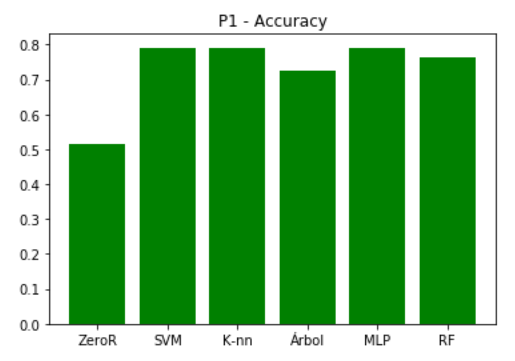
\includegraphics[width=43mm]{imagenes/p1_acc}}
  \subfigure[F1-Score]{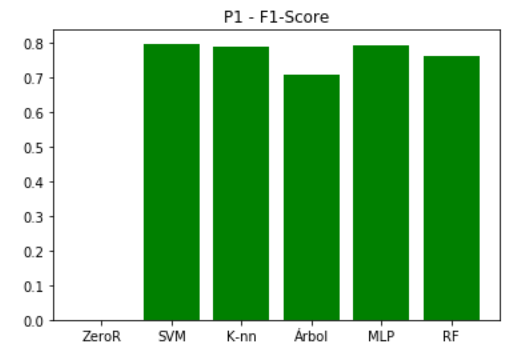
\includegraphics[width=43mm]{imagenes/p1_f1}}
  \subfigure[TPR]{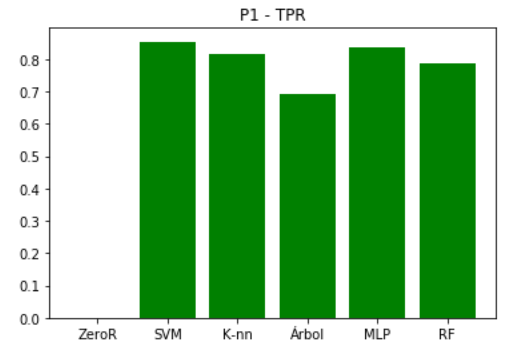
\includegraphics[width=43mm]{imagenes/p1_tpr}}
  \subfigure[FNR]{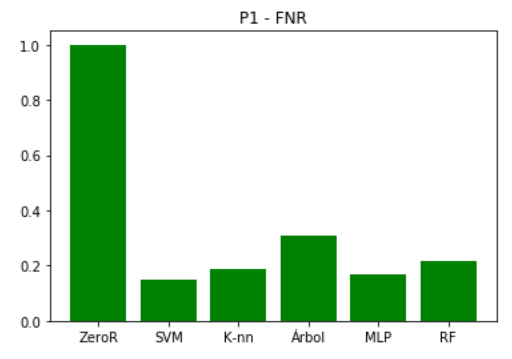
\includegraphics[width=43mm]{imagenes/p1_fnr}}
\end{figure}

\vspace{-5mm}

\begin{center}
  \textbf{Procesado 2}
\end{center}

\begin{figure}[H]
  \centering
  \subfigure[Accuracy]{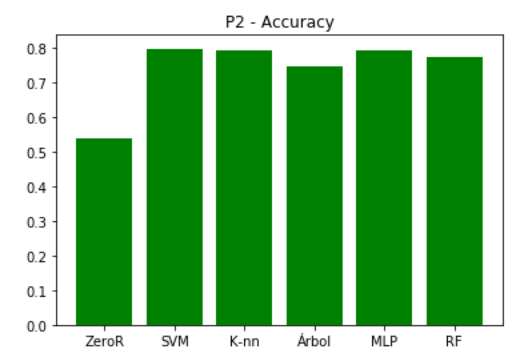
\includegraphics[width=43mm]{imagenes/p2_acc}}
  \subfigure[F1-Score]{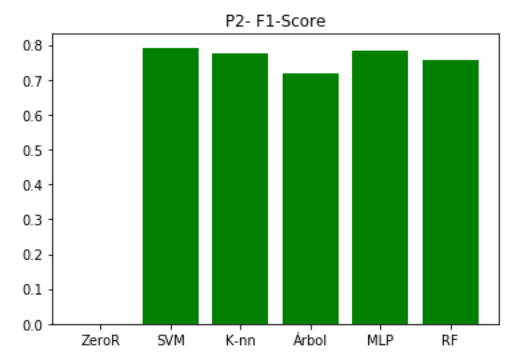
\includegraphics[width=43mm]{imagenes/p2_f1}}
  \subfigure[TPR]{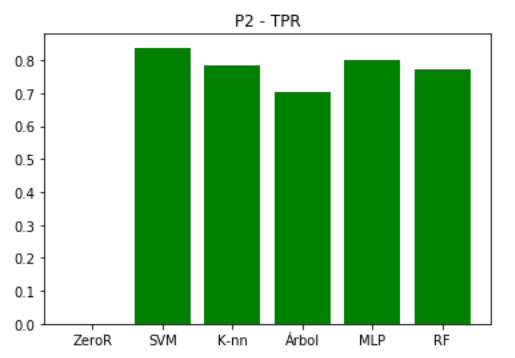
\includegraphics[width=43mm]{imagenes/p2_tpr}}
  \subfigure[FNR]{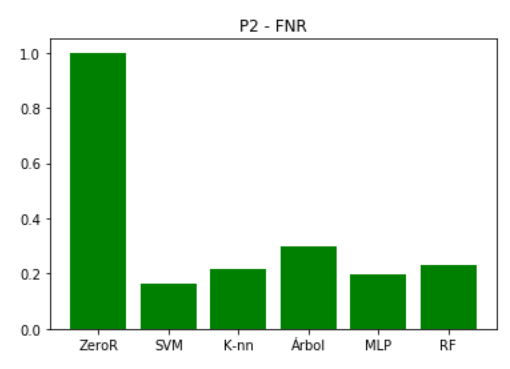
\includegraphics[width=43mm]{imagenes/p2_fnr}}
\end{figure}

\vspace{-5mm}

\begin{center}
  \textbf{Procesado 3}
\end{center}

\begin{figure}[H]
  \centering
  \subfigure[Accuracy]{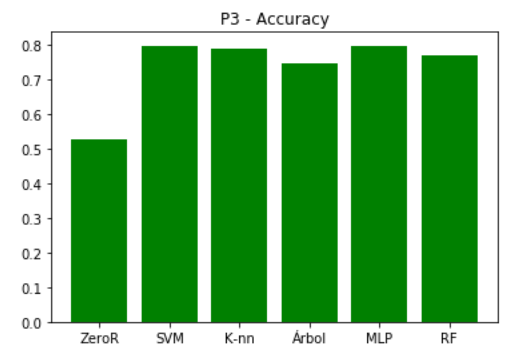
\includegraphics[width=43mm]{imagenes/p3_acc}}
  \subfigure[F1-Score]{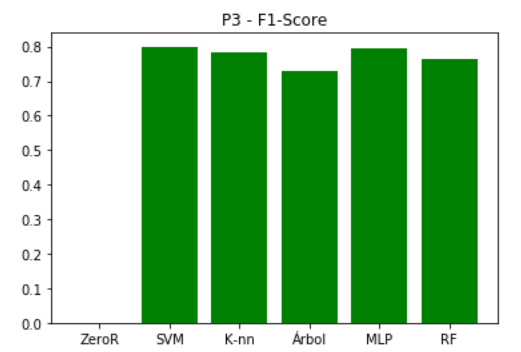
\includegraphics[width=43mm]{imagenes/p3_f1}}
  \subfigure[TPR]{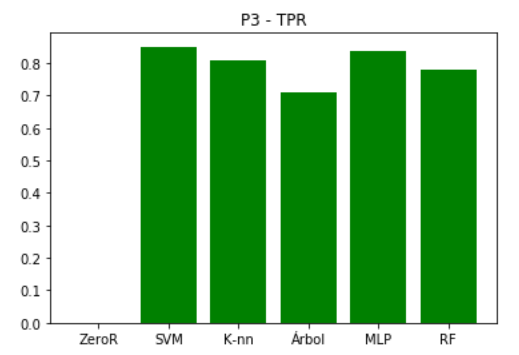
\includegraphics[width=43mm]{imagenes/p3_tpr}}
  \subfigure[FNR]{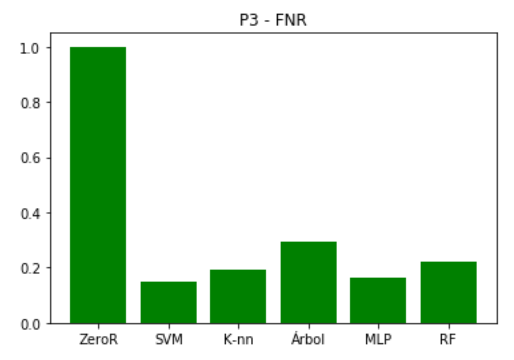
\includegraphics[width=43mm]{imagenes/p3_fnr}}
\end{figure}

\vspace{-5mm}

El código de cada gráfica es:

\begin{lstlisting}
fig, ax = plt.subplots()
ax.bar(["ZeroR", "SVM", "K-nn", "Arbol", "MLP", "RF"], pX_metrica, color='green')
ax.set_title("PX-metrica")
\end{lstlisting}

Donde ``X'' es denota el preprocesado que se ha aplicado, $1, 2$ o $3$, y `` metrica'' la métrica que se mide, pudiendo ser \texttt{accuracy}, \texttt{F1-Score}, \texttt{TPR} o \texttt{FNR}. El vector pX-metrica es un vector donde se guardan los valores de la métrica ``metrica'' con el preprocesado ``X'' de todos los modelos considerados.

Podemos observar que los tres preprocesados obtienen resultados muy similares, como ya comentamos en la práctica anterior. A primera vista, la estructura de los diagramas parece la misma, es decir, al ordenar los diferentes modelos según el valor de la métrica correspondiente con cada procesamiento, este orden es muy parecido en todos ellos, no atreviéndome a decir el mismo por haber barras de alturas semejantes. Es por esto que decantarse por un procesamiento con estos gráficos resulta complicado.

En los tres preprocesamientos el modelo con menor \texttt{accuracy} es el ZeroR, seguido del árbol de decisión. El SVM, K-nn y MLP son los modelos con mayor \texttt{accuracy} en los tres casos. En el resto de métricas se obserba que el SVM y el MLP tienen un mejor desempeño que el K-nn, siendo estos dos modelos los que mejores resultados obtienen. El árbol de decisión y el ZeroR son los modelos que peor desempeño tienen. El Random Forest y el árbol de decisión no obtienen tan buenos resultados como los otros modelos inicialmente pero, como vimos en la práctica 1, aplicando la poda coste-complejidad obteniamos una gran mejora de su desempeño, ya que con esta poda se conseguía reducir el sobreajuste del modelo.

Para elegir que procesamiento utilizabamos en la práctica 1, nos decantamos por el procesamiento que en más modelos tuviese mayor \texttt{F1-Score}. En las siguientes gráficas mostramos el valor de esta métrica en los diferentes modelos para cada procesamiento: 

\begin{figure}[H]
  \centering
  \subfigure[ZeroR]{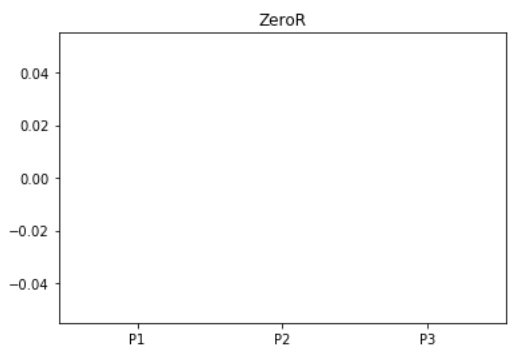
\includegraphics[width=57mm]{imagenes/zeror}}
  \subfigure[SVM]{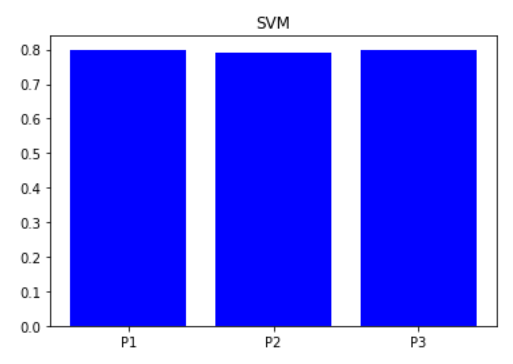
\includegraphics[width=57mm]{imagenes/svm}}
  \subfigure[k-nn]{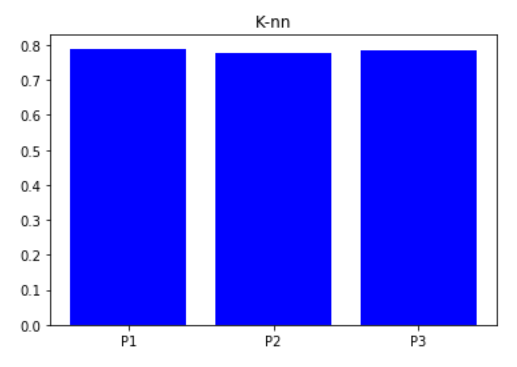
\includegraphics[width=57mm]{imagenes/knn}}
\end{figure}

\begin{figure}[H]
  \centering
  \subfigure[Árbol de decisión]{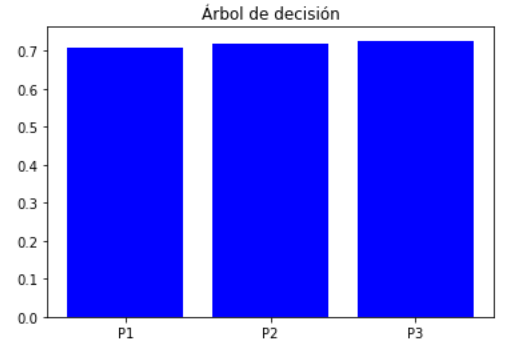
\includegraphics[width=58mm]{imagenes/arbol}}
  \subfigure[MLP]{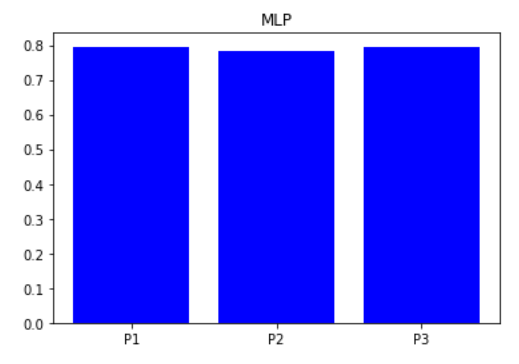
\includegraphics[width=55mm]{imagenes/mlp}}
  \subfigure[Random Forest]{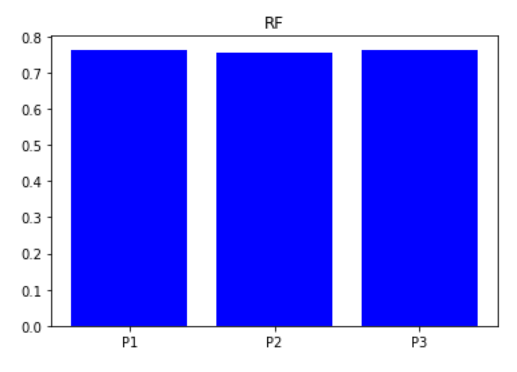
\includegraphics[width=60mm]{imagenes/rf}}
\end{figure}

Como ya hemos visto antes, no hay gran diferencia entre unos y otros. En el modelo ZeroR la \texttt{F1-Score} es $0$ en los tres casos, debido a que etiqueta todas las muestras como negaticas, luego no hay verdaderos positivos. En los modelos SVM, MLP, Random Forest y K-nn el procesamiento de datos 2 parece tener resultados ligeramente inferiores que los otros dos, que están muy igualados. En el árbol de decisión el procesamiento 2 tiene un mejor desempeño que el 1, pero peor que el 3. Este modelo es el que peores resultados ofrece sin considerar el ZeroR. Como podemos obsservar que el eje $Y$ no llega a $0.8$ como en los demás.

Al igual que en la práctica 1, el procesado de datos  que usaría usando la información recogida en estas gráficas sería el procesado 3, porque en el árbol de decisión se ve que es el que mejores resultados ofrece y en el resto de modelos la diferencia con el procesado 1 no puedo apreciarla a simple vista.

Para crear las gráficas primero se crearon para cada modelo vector que contiene el valor de la métrica \texttt{F1-Score} de cada uno de los preprocesados:

\begin{lstlisting}
v_zeror = [p1_f1[0], p2_f1[0], p3_f1[0]]
v_svm   = [p1_f1[1], p2_f1[1], p3_f1[1]]
v_knn   = [p1_f1[2], p2_f1[2], p3_f1[2]]
v_arbol = [p1_f1[3], p2_f1[3], p3_f1[3]]
v_mlp   = [p1_f1[4], p2_f1[4], p3_f1[4]]
v_rf    = [p1_f1[5], p2_f1[5], p3_f1[5]]
\end{lstlisting}

Tras esto, para cada uno de los modelos creamos la gráfica correspondiente así:

\begin{lstlisting}
fig, ax = plt.subplots()
ax.bar(["P1", "P2", "P3"], v_clf, color='blue')
ax.set_title("clf")
\end{lstlisting}

donde ``clf'' denota el clasificador del que recogemos los datos en la gráfica.  

\subsection{Curva ROC}

Para representar la curva ROC dividimos el conjunto de datos al que se le ha aplicado el procesado 3 salvo la normalización en comjunto de entrenamiento y conjunto de validación. La división se hace de manera que el $70\%$ de los datos formen el conjunto de entrenamiento y el otro $30\%$, el de test, conservando la proporción de elementos en cada clase tanto en el conjunto de entrenamiento como en el de validación. Esto se hace con el código:

\begin{lstlisting}
  X_train, X_test, y_train, y_test = model_selection.train_test_split(data, target,
  test_size=0.3, stratify=target, random_state=0)
\end{lstlisting}

Tras esto,, completamos el procesado de datos $3$ usando \texttt{MinMaxScaler()} para normalizar los datos de entrenamiento y se usa estas mismas transformaciones sobre los datos de validación. A continuación, entrené los modelos con los hiperparámetros seleccionados en la práctica anterior. Podemos representar en una gráfica la curva ROC de los diferentes modelos así:

\begin{lstlisting}
ax = plt.gca()

for model in [dummy_clf, svm_clf, knn_clf, tree_clf, mlp_clf, rf_clf]:
    metrics.plot_roc_curve(model, data, target, ax=ax)  
\end{lstlisting}

El resultado es:

\begin{figure}[H]
  \centering
  \caption{Curva ROC}
  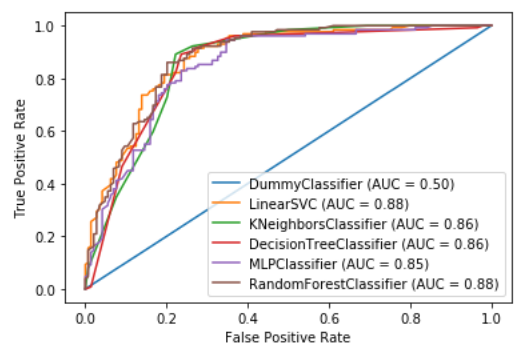
\includegraphics[width=131mm]{imagenes/ROC}
\end{figure}

Los modelos que presentan mayor métrica \texttt{AUC} son el Random Forest y el SVM, que son aquellos con mayor área bajo la curva ROC y los que tienen una mayor pendiente en los valores cercanos al cero. Esto implica que estos clasificadores son capaces de incrementar el número de verdaderos positivos a un ritmo mayor que el número de falsos positivos. Si usásemos esta métrica para sacar conclusiones, éstos serían los mejores modelos, mientras que el  MLP es el modelo que peor comportamiento muestra, excluyendo al ZeroR. A pesar de esto, no hay excesivas diferencias entre los modelos considerados, a excepción del ZeroR.

\subsection{Análisis de los atributos}

En esta sección estudiaremos la importancia de los diferentes atributos en la clasificación. Para ello se visualizarán gráficos de barras para cada uno de los diferentes atributos y para cada una de las etiquetas, de manera que se muestre la distribución de los valores que toma dicho atributo en función de su etiqueta. También visualizaremos los diagramas de cajas, ``boxplots'', de aquellos atributos donde tenga sentido.\\

Empezamos mostrando las gráficas correspondientes al atributo \texttt{BI-RADS}:

\begin{figure}[H]
  \centering
  \caption{Cantidad de datos con cada etiqueta}
  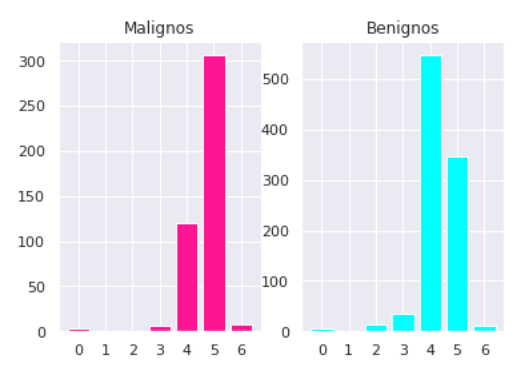
\includegraphics[width=100mm]{imagenes/bi_rads}
\end{figure}

Este atributo representa la opinión de un médico experto sobre la gravedad del tumor. Si tiene el valor ``1'' o ``2'', el tumor es benigno, del mismo modo, si toma el valor ``6'' es maligno. Los valores ``3'', ``4'' y ``5'' designan casos en los que no se está seguro de la severidad del tumor, pero hay cierta probabilidad de que sea maligno o benigno. Esta información la podemos comprobar en \href{https://es.wikipedia.org/wiki/BI-RADS}{https://es.wikipedia.org/wiki/BI-RADS}. Este atributo da mucha información sobre la naturaleza del tumor, pero dado que necesitamos la opinión de un experto para obtenerlo, no es apropiado usarlo para el aprendizaje.

Según la página \href{https://bigml.com/user/TotyB/gallery/dataset/509a98c6035d0706dd0001dd}{https://bigml.com/user/TotyB/gallery/dataset/509a98c6035d0706dd0001dd}, de donde hemos obtenido los datos, el $94.46\%$ de estos tienen \texttt{BI-RADS} ``4'' o ``5''. De estos, los tumores con valor ``5'' son probablemente malignos. Los tumores malignos tienen más variabilidad que los benignos, dado que hay tumores malignos con valor de \texttt{BI-RADS} ``4'' o ``5'', predominando el valor ``5''. En el caso de los benignos, la mayoría de estos tienen la categoría de \texttt{BI-RADS} ``4''.

Esto se ve en el diagrama de cajas de este atributo:

\begin{figure}[H]
  \centering
  \caption{Diagrama de cajas de BI-RADS}
  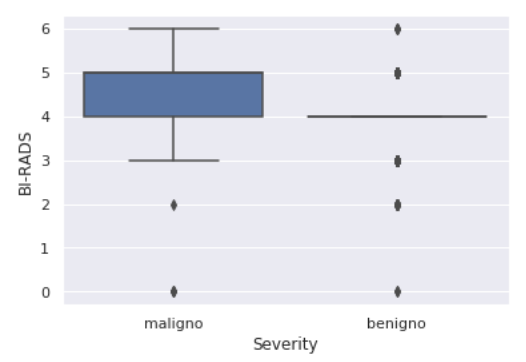
\includegraphics[width=100mm]{imagenes/bp_birads}
\end{figure}

Los tumores etiquetados como malignos se mueven entre el valor ``4'' o ``5'' mientras que la mayoría de los benignos toman el valor ``4''.

La gráfica del atributo edad nos proporciona los siguientes resultados:

\begin{figure}[H]
  \centering
  \caption{Cantidad de datos con cada etiqueta}
  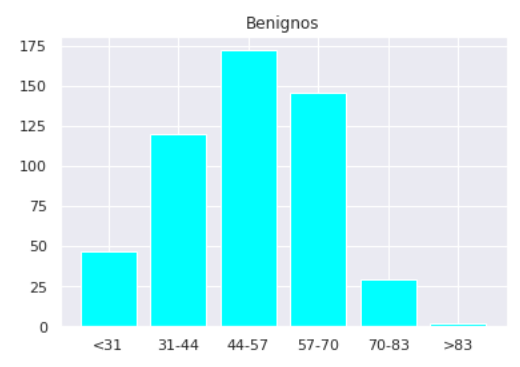
\includegraphics[width=87mm]{imagenes/edad_ben}
  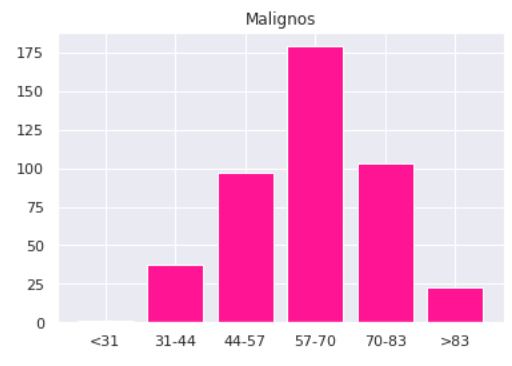
\includegraphics[width=87mm]{imagenes/edad_mal}
\end{figure}

Vemos que cuanto menor edad tiene una persona, más probable es que su tumor sea benigno. En particular, la mayoría de las personas menores de $31$ años de la muestra tienen tumores benignos y gran parte de las que tienen más de $83$ tienen tumores malignos. En el diagrama de cajas podemos observar que la mediana de edad de los pacientes con tumores malignos de la muestra es superior a los $60$ años, mientras que la de los pacientes con tumores benignos está rondando los $50$. Aunque la edad de los pacientes con tumores benignos varía entre los $18$ y algo más de los $80$ años, los datos entre el primer y el tercer cuartil se encuentran concentrados entre los $40$ y $60$. Los datos entre el primer y el tercer cuartil de los tumores malignos se encuentran entre algo más de los $50$ y algo más de los $70$ años.

Por consiguiente, la edad de una persona sí es un atributo relevamte en la clasificación, porque aunque no podríamos estimar la severidad del tumor sabiendo sólo la edad de ésta, si una persona es muy joven podríamos esperar que su tumor sea benigno. 

\begin{figure}[H]
  \centering
  \caption{Diagrama de cajas de la edad}
  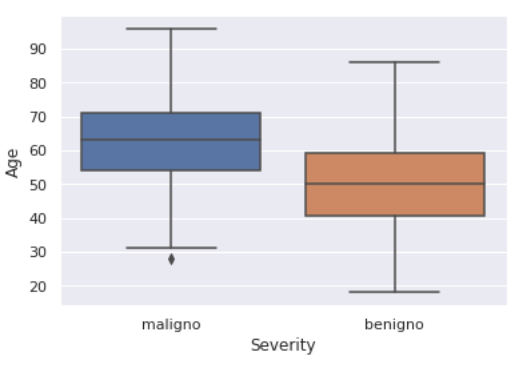
\includegraphics[width=87mm]{imagenes/bp_age}
\end{figure}

A continuación, analizaremos las gráficas del atributo Shape. La mayoría de los tumores malignos tienen una forma irregular, mientras que los benignos suelen tener una forma ovalada o redondeada. Los tumores benignos presentan mayor variabilidad en los valores que toman en este atributo que los malignos. Resulta interesante considerar este atributo para nuestro aprendizaje, ya que la distribución de los valores que toman los tumores malignos difiere bastante de la de los benignos.\\

\begin{figure}[H]
  \centering
  \caption{Cantidad de datos con cada etiqueta}
  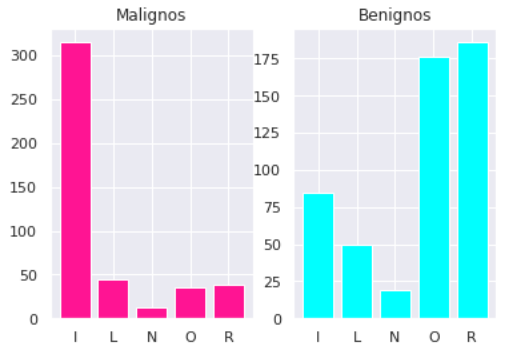
\includegraphics[width=87mm]{imagenes/shape}
\end{figure}

Como el atributo Shape es cualitativo y no tiene orden, no tiene sentido dibujar un diagrama de cajas en este caso, ya que este variaría para cada asignación diferente de valores numéricos a cada posible valor del atributo, y esta asignación es totalmente aleatoria, ya que estos carecen de orden.\\

El siguiente atributo a analizar es Margin. Al igual que en Shape, los distintos valores que toma este atributo no tienen un orden determinado, por lo tanto no representé el diagrama de cajas de este atributo. Los tumores malignos tienen mayor variabilidad que los benignos, siendo el valor de Margin más frecuente entre estos ``ill-defined'' seguido del ``spiculated''. Los benignos, sin embargo, suelen tener margin ``circumscribed''. En la práctica 1, una vez eliminados los atributos \texttt{BI-RADS} y Density, vimos que este atributo era el que mayor información nos aportaba en la clasificación, dado que era el elegido en el nodo raíz del árbol de decisión. Aquí podemos comprobar que efectivamente hay una gran diferencia entre la distribución de los valores de Margin que toman los tumores malignos de los benignos, cosa que afecta favorablemente a la clasificación, permitiéndonos diferenciar una muestra maligna de una benigna con mayor facilidad.

\begin{figure}[H]
  \centering
  \caption{Cantidad de datos con cada etiqueta}
  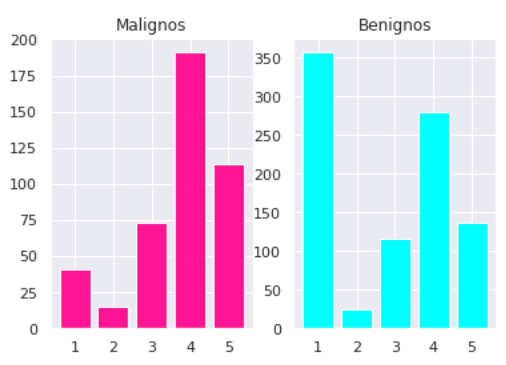
\includegraphics[width=87mm]{imagenes/margin}
\end{figure}

Por último, analizamos el atributo Density. Como ya comentamos, este atributo tiene muy poca variabilidad en la muestra y podemos comprobar que los dos diagramas de barras son muy parecidos, lo que nos incita a pensar que este atributo no aporta apenas información a la clasificación.

\begin{figure}[H]
  \centering
  \caption{Cantidad de datos con cada etiqueta}
  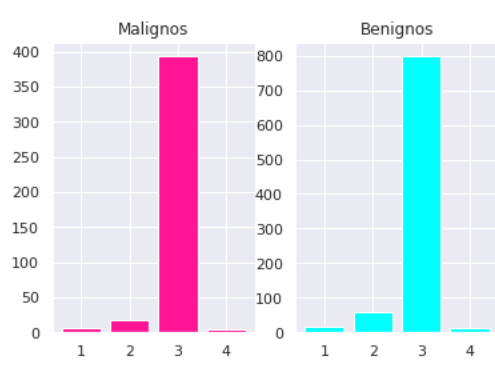
\includegraphics[width=87mm]{imagenes/density}
\end{figure}

En el diagrama de cajas volvemos a apreciar la poca variabilidad de este atributo, ya que cualquier valor distinto de $3$ lo interpreta como outlayer. Esta razón fue la que me llevó a considerar eliminar este atributo durante el procesado de datos $3$.

\begin{figure}[H]
  \centering
  \caption{Diagrama de cajas de Density}
  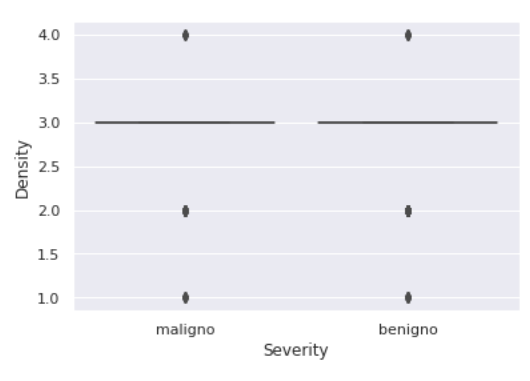
\includegraphics[width=65mm]{imagenes/bp_density}
\end{figure}

\section{Segmentación}

\subsection{Introducción}

El problema que abordaremos en esta sección es agrupar accidentes obtenidos de los datos publicados por la Dirección General de Tráfico  en conjuntos de accidentes con características similares. Para ello utilizaremos técnicas de clustering estudiadas en la asignatura, concretamente \texttt{K-means} y \texttt{DBSCAN}. Ambos métodos son métodos de particionamiento.

El algortimo \texttt{K-means} necesita como parámetro el número de clústers deseado y va clasificando las diferentes instancias en el clúster cuyo centroide sea el más cercano a ésta. Es un método iterativo que recalcula el centroide en cada iteración y repite el proceso de clasificación de las instancias. Termina cuando en una iteración ninguna instancia cambia de clúster. El algoritmo siempre converge.

El algoritmo \texttt{DBSCAN} depende de los parámetros \textit{epsilon} y \textit{min\_samples}. El primero indica la distancia máxima a la que se considera que dos puntos son directamente alcanzables. Para que un punto sea un punto núcleo necesita que haya al menos \textit{min\_samples} a distancia menor que \textit{epsilon} de él. A partir de ahí, un punto será alcanzable si existe una secuencia de puntos $p_1, \ldots, p_n$ tales que $p_{i+1}$ es directamente alcanzable desde $p_i$. Cada punto núcleo forma un clúster formado por todos aquellos puntos alcanzables desde él. A los puntos que no pertenecen a ningún clúster se les asigna el clister $-1$.

Los atributos en los que nos basamos para hacer la segmentación son:

\begin{itemize}
\item \texttt{TOT\_VICTIMAS}: Total de víctimas
\item \texttt{TOT\_MUERTOS}: Total de muertos
\item \texttt{TOT\_HERIDOS\_GRAVES}: Total de heridos graves.
\item \texttt{TOT\_HERIDOS\_LEVES}: Total de heridos leves.
\item \texttt{TOT\_VEHICULOS\_IMPLICADOS}: Total de vehículos involucrados en el accidente.
\end{itemize}

Las métricas que usaremos para la estimar la bondad del ajuste son el coeficiente Silhouette y el índice Calinski-Harabasz.

El coeficiente Silhouette mide como de similares son los elementos del mismo clúster comparado con los elementos de otro clúster. Este coeficiente es la media de los $s(i)$, con

$$s(i) = \frac{b(i)-a(i)}{\max\{a(i), b(i)\}}$$

donde $b(i)$ es la mínima distancia del elemento $i$ a otro clúster y $a(i)$ es la distancia media del elemento al resto de instancias de su clúster. Cuanto mayor sea este coeficiente, mejor es el rendimiento del modelo.

El índice Calinski-Harabasz mide la razón entre la dispersión interclústers y la dispersión intraclústers. El agrupamiento será mejor cuanto mayor sea este índice.

Para la elección de hiperparámetros, elegiremos aquellos que maximicen el índice Calinski-Harabasz, que utiliza todas las muestras para su cálculo y dado que usamos los mismos datos en todas las iteraciones, que su valor no esté normalizado no afecta en la interpretación del resultado.

Antes de realizar el análisis ejecutando los algoritmos de clusterig normalizamos los datos con la función \texttt{MinMaxScaler}, cuyo comportamiento es el mismo que la función \texttt{norm} de \texttt{pract2\_utils}, por lo que es correcto usar \texttt{denorm} con los datos normalizados para deshacer esta operación (como hacemos para representar los centroides).

\newpage
\subsection{Caso de estudio 1: Choque frontal en carreteras convencionales}

Estudiaremos las propiedades de los choques frontal en carreteras convencionales que, según el libro \href{https://www.todostuslibros.com/libros/manual-del-alumno-permiso-b-facilauto_978-84-09-08551-4}{Manual del alumno. Permiso B}, es el caso de accidente con más víctimas mortales. Por tanto estudiaremos las diferentes características de dichos accidentes mediante clustering, agrupando los accidentes de esta caterogía y viendo las propiedades de cada uno de esos grupos. Para ello usaremos los algoritmos K-Means y DBSCAN.

\subsubsection{K-means}

El algoritmo \texttt{K-means} tiene como parámetro el número de clústers a considerar. Para elegir el mejor valor de éste, ejecuté el algoritmo con un número de clústers comprendido entre $2$ y $14$. Los resultados de las métricas son:

\begin{center}
\begin{tabular}{|c|c|c|}
\hline
\multicolumn{1}{|c|}{\textbf{Nº de clústers}}& \textbf{Silhouette} & \textbf{Calinski-Harabasz}\\ \hline
  2  & 0.4755151052183165  & 637.8831140088855  \\ \hline
  3  & 0.46599969633063965 & 597.9798532808658  \\ \hline
  4  & 0.48348908673333896 & 634.4016355078425  \\ \hline
  5  & 0.531569055229591   & 683.2263367508311  \\ \hline
  6  & 0.5404576589330072  & 646.8004817570682  \\ \hline
  7  & 0.5519986909803548  & 630.8036708742871  \\ \hline
  8  & 0.5786471085948179  & 634.4445453990445  \\ \hline
  9  & 0.5903779353773022  & 628.3756258948337  \\ \hline
 10  & 0.6461326222918197  & 659.4342926638305  \\ \hline
 11  & 0.6893747693555886  & 653.852874658656   \\ \hline
 12  & 0.7336714808160643  & 659.3965542394021  \\ \hline
 13  & 0.744841516853055   & 665.0690582901761  \\ \hline
 14  & 0.749410469848095   & 663.5502144820157  \\ \hline
\end{tabular}
\end{center}

Para facilitar la comprensión de la tabla, visualizamos la información que contiene en las siguientes gráficas, que se realizan utilizando la función \texttt{grafica}, cuyo código es:

\begin{lstlisting}
def grafica(data, label, title, xlab, ylab):
    plt.plot(data,label, c='b')
    plt.title(title)
    plt.xlabel(xlab)
    plt.ylabel(ylab)

    plt.show()
  \end{lstlisting}

Obtenemos el siguiente resultado:

\begin{figure}[H]
  \centering
  \caption{Gráficas con el valor de las métricas en función del número de clústers}
  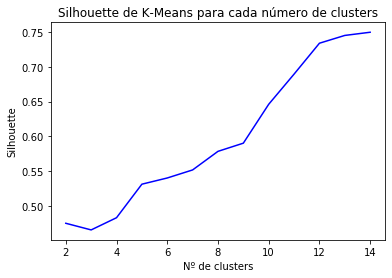
\includegraphics[width=87mm]{imagenes/c1_kmeans_sil}
  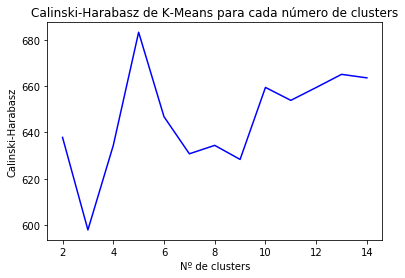
\includegraphics[width=87mm]{imagenes/c1_kmeans_cal}
\end{figure}

Vemos que el coeficiente Calinski-Harabasz alcanza un máximo cuando se consideran 5 clústers, por lo que elegiremos este valor para dicho hiperparámetro.

El resultado de la segmentación es la división del conjunto de accidentes considerados en 5 conjuntos con las siguiente distribución:

\begin{figure}[H]
  \centering
  \caption{Clústers}
  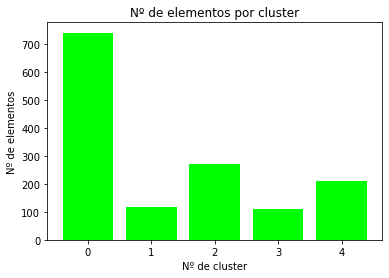
\includegraphics[width=100mm]{imagenes/c1_kmeans_clusters}
\end{figure}

Vemos que el $51.24\%$ de los accidentes pertenecen al clúster $0$. El siguiente clúster más grande, el $2$, posee el $18.65\%$ de éstos y el $4$ posee el $14.51\%$. Los clústers con menos elementos son el $1$ y el $3$ con el $8.08\%$ y el $7.53\%$, respectivamente. Veremos después las características de cada uno de los clústers.

Los valores de las métricas para este modelo son:

\begin{center}
\begin{tabular}{|c|c|}
\hline
\multicolumn{1}{|c|}{\textbf{Silhouette}} & \textbf{Calinski-Harabasz}\\ \hline
 0.531569055229591   & 683.2263367508311  \\ \hline
\end{tabular}
\end{center}

Los centroides de los diferentes clusters son:

\begin{figure}[H]
  \centering
  \caption{Centroides}
  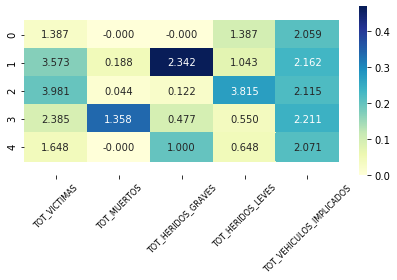
\includegraphics[width=120mm]{imagenes/c1_kmeans_centroides}
\end{figure}

El clúster $0$, que es aquel con más instancias, tiene como centro un accidente con $2.059$ vehículos implicados, del que $1.387$ personas han sido heridos leves, pero sin muertos ni heridos graves. Es el clúster cuyo centro tiene un menor número de víctimas, y las que tiene son heridos leves. Podemos deducir que en este clúster estarán accidentes sin heridos graves ni muertos, y aunque el número de heridos leves varíe, hay más accidentes con un sólo herido leve.

El clúster $1$ tiene como centro un accidente con $3,573$ víctimas, en el que $2,342$ son heridos graves, $1.043$ son heridos leves y $0.188$ son muertos. Hubo $2.162$ vehículos implicados. Es el clúster con mayor número de heridos graves de media, pero es el segundo clúster con menos instancias. Por tanto vemos que el número de accidentes con muchos heridos graves no es tan alto como el número de accidentes con un sólo herido leve.

El clúster $2$ tiene como centro un accidente con $3.981$ víctimas, la mayoría heridos leves. Tiene de media más víctimas y heridos leves que el resto, pero es el segundo con menos heridos graves. Como en el resto de clústers, los vehículos involucrados están alrededor de $2$. Por tanto, podemos esperar que en este clúster haya instancias con un gran número de heridos leves, pero sin muertos o heridos graves en la mayoría de ellos.

El clúster $3$ tiene como centro un accidente con $2.3850$ víctimas. Tiene de media más muertos que el resto, $1.358$ muertos. También tiene $0.477$ heridos graves y 0.55 heridos leves. El el clúster con menos instancias de los cinco. Por tanto, esperamos que este clúster sea el que tenga los accidentes donde hay muertos, pero el número de muertos medio es más cercano a uno que a dos, luego la mayoría tendrán sólo un muerto.

El clúster 4 tiene como centro un accidente con $1.648$ víctimas, pero ningún muerto. Es el segundo clúster con más heridos graves y el segundo con menos heridos leves. Como en el resto de clústers, el número de vehículos implicados está entorno a dos. Podemos deducir que la mayoría de accidentes de este clúster tienen entre cero y un herido leve y un herido grave.

Las diferencias entre los distintos clústers pueden visualizarse con \texttt{pairplot}:

\begin{figure}[H]
  \centering
  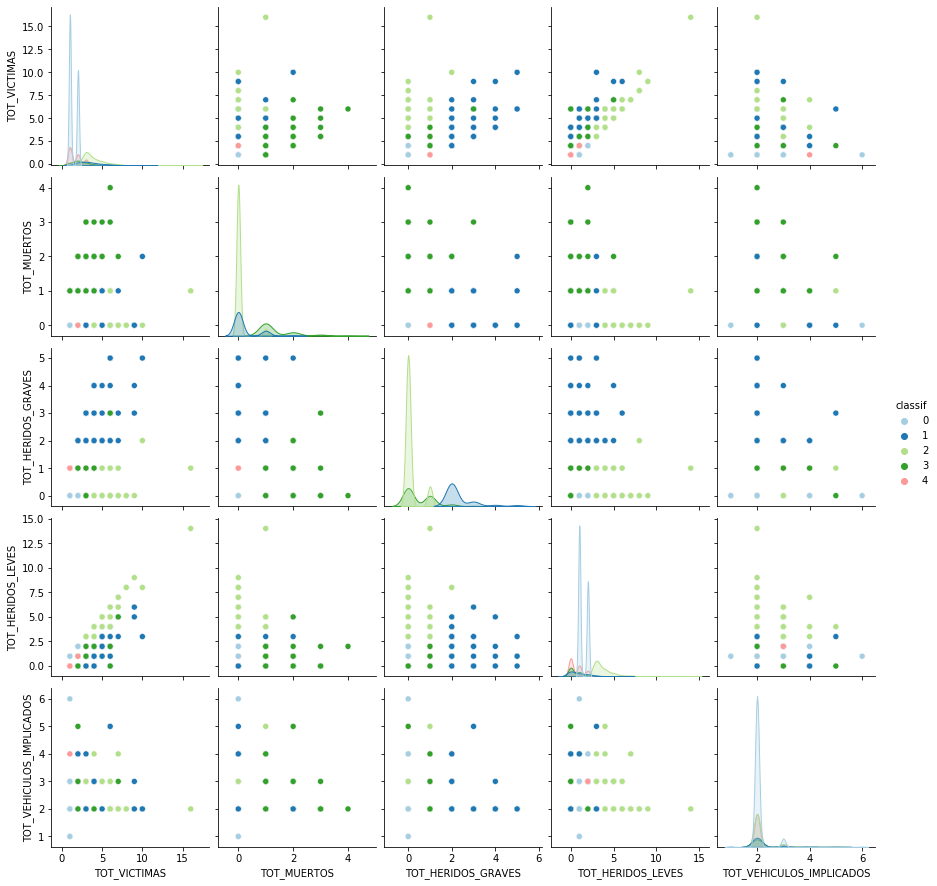
\includegraphics[width=140mm]{imagenes/c1_kmeans_pairplot}
\end{figure}

Podemos corroborar lo que vimos con los centroides, que todos los clústers suelen tener entorno a 2 vehículos implicados. También observamos que el atributo \texttt{TOT\_VICTIMAS} es directamente proporcional a los atributos \texttt{TOT\_HERIDOS\_GRAVES}, \texttt{TOT\_HERIDOS\_LEVES} y \texttt{TOT\_MUERTOS}. En el atributo \texttt{TOT\_HERIDOS\_GRAVES} nos ayuda a discernir el clúster 1 de los clusters 2 y 3, ya que podemos ver que las distribuciones de este atributo en los clústers son distintas. El atributo \texttt{TOT\_HERIDOS\_LEVES} diferencia los clústers 4, 0 y 2. Para ver estas diferencias de manera más detallada podemos usar \texttt{boxplot}:

\begin{figure}[H]
  \centering
  \caption{Diagramas de cajas}
  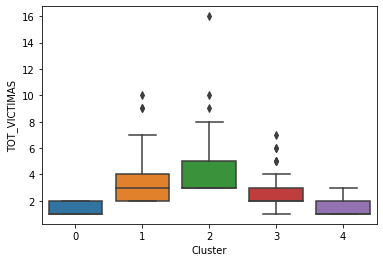
\includegraphics[width=87mm]{imagenes/c1_kmeans_bp_vic}
  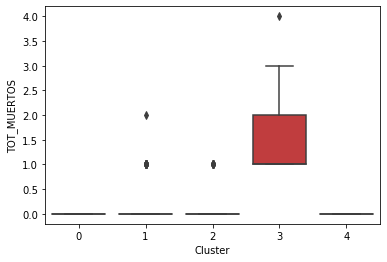
\includegraphics[width=87mm]{imagenes/c1_kmeans_bp_muertos}
    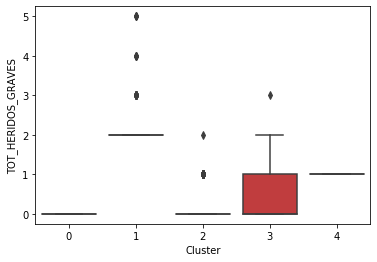
\includegraphics[width=87mm]{imagenes/c1_kmeans_bp_hg}
  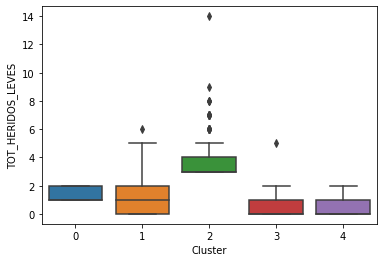
\includegraphics[width=87mm]{imagenes/c1_kmeans_bp_hl}
  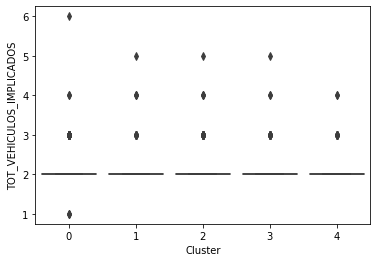
\includegraphics[width=87mm]{imagenes/c1_kmeans_bp_vi}
\end{figure}

\newpage
En la siguiente tabla mostramos el rango de valores más representativo de cada cluster:

\begin{center}
\begin{tabular}{|c|c|c|c|c|c|}
\hline
\multicolumn{1}{|c|}{\textbf{Nº del clúster}} & \textbf{Víctimas} & \textbf{Muertos} & \textbf{Heridos graves} & \textbf{Heridos leves} & \textbf{Vehículos implicados}\\ \hline
  0  & 1-2 & 0   & 0   & 1-2 & 2 \\ \hline
  1  & 2-7 & 0   & 2   & 0-5 & 2 \\ \hline
  2  & 3-8 & 0   & 0   & 3-5 & 2 \\ \hline
  3  & 0-4 & 1-3 & 0-2 & 1-2 & 2 \\ \hline
  4  & 0-3 & 0   & 1   & 1-2 & 2 \\ \hline
\end{tabular}
\end{center}

Salvo outlayers, todos los clúster están compuestos por accidentes con dos vehículos implicados.

El clúster $0$ está compuesto por accidentes sin muertos ni heridos graves, y entre uno y dos heridos leves. Es aquel con más datos y cuyos accidentes son menos graves.

El clúster $1$ está formado principalmente por accidentes con dos heridos graves y entre cero y cinco heridos leves. Es aquel con mayor variabilidad de heridos leves.

El clúster $2$ está compuesto mayoritariamente por accidentes sin muertos ni heridos graves y entre tres y cinco heridos leves. Es aquel con más víctimas, pero todas ellas son heridos leves.

El clúster $3$ es el único cluster, salvo oultayers, en cuyos accidentes hay muertos, entre uno y cinco concretamente. hay entre cero y dos heridos graves y entre uno y dos leves.

El clúster $4$ se compone de accidentes con un herido grave y entre uno y dos leves.

Vemos que el atributo \texttt{TOT\_VEHICULOS\_IMPLICADOS} no es muy informativo, ya que todos los clústers se componen mayoritariamente de accidentes donde sólo hay dos vehículos implicados. El atributo \texttt{TOT\_MUERTOS} sólo ayuda a diferenciar un clúster del resto. Los atributos que más información dan sobre la composición de cada clúster son \texttt{TOT\_HERIDOS\_LEVES} y \texttt{TOT\_HERIDOS\_GRAVES}.

\subsubsection{DBSCAN}

El algoritmo DBSCAN tiene como parámetro la distancia a la que consideramos que dos puntos son directamente alcanzables, \textit{epsilon}. Consideré que un clúster tenía que estar constituido por 10 puntos mínimo. Para elegir el mejor valor de \textit{epsilon}, ejecuté el algoritmo con diez valores de \textit{epsilon} equidistantes entre 0.02 y 0.2, ambos incluidos. Elegí valores inferiore a 0.2 porque con valores mayores de \textit{epsilon} el algoritmo sólo creaba un clúster diferente al clúster $-1$.  Los resultados de las métricas son:

\begin{center}
\begin{tabular}{|c|c|c|}
\hline
\multicolumn{1}{|c|}{\textbf{Epsilon}}& \textbf{Silhouette} & \textbf{Calinski-Harabasz}\\ \hline
  0.02  & 0.7895289623335725  & 114.4553269039885  \\ \hline
  0.04  & 0.7895289623335725  & 114.4553269039885  \\ \hline
  0.06  & 0.7895289623335725  & 114.4553269039885  \\ \hline
  0.08  & 0.7895289623335725  & 114.4553269039885  \\ \hline
  0.1   & 0.4869805568764864  & 165.50098317272966  \\ \hline
  0.12  & 0.4869805568764862  & 165.50098317272966  \\ \hline
  0.14  & 0.4869805568764861  & 165.50098317272966  \\ \hline
  0.16  & 0.4869805568764864  & 165.50098317272966  \\ \hline
  0.18  & 0.4869805568764862  & 165.50098317272966  \\ \hline
  0.2   & 0.5005453962094687  & 185.66574970475563  \\ \hline
\end{tabular}
\end{center}

Para facilitar la comprensión de la tabla, visualizamos la información que contiene en las siguientes gráficas:

\begin{figure}[H]
  \centering
  \caption{Gráficas con el valor de las métricas en función del número de clústers}
  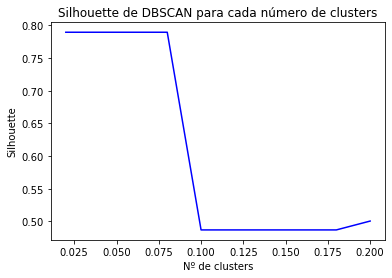
\includegraphics[width=73mm]{imagenes/c1_dbscan_sil}
  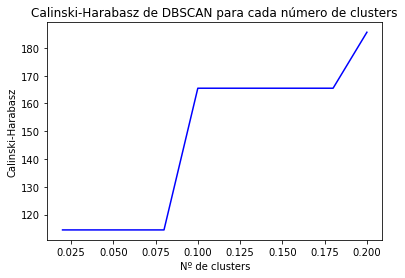
\includegraphics[width=73mm]{imagenes/c1_dbscan_cal}
\end{figure}

Para elegir el valor de \textit{epsilon} apropiado, visualizamos los clústers formados con \textit{epsilon}$ = 0.08$ y \textit{epsilon}$=0.1$:

\begin{figure}[H]
  \centering
  \caption{Gráficas con \textit{epsilon} = 0.08 y \textit{epsilon}=0.1 respectivamente}
  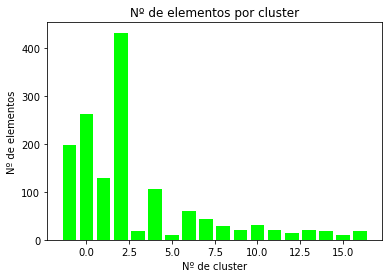
\includegraphics[width=73mm]{imagenes/c1_dbscan_cluster_008}
  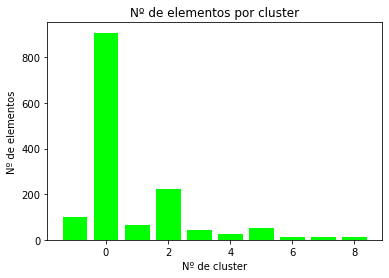
\includegraphics[width=73mm]{imagenes/c1_dbscan_cluster_01}
\end{figure}

Elegimos el valor de \textit{epsilon}$ = 0.1$, dado que con \textit{epsilon}=0.08 trece de los diecisiete clústers formados tienen menos de 60 datos. Además, hay casi el doble de accidentes componiendo el clúster $-1$, es decir, hay casi el doble de elementos que no han podido asignarse a ninguno de los otros clústers y no tienen un clúster que los represente. Por tanto, la distribución de los clústers con el parámetro ajustado es:

\begin{figure}[H]
  \centering
  \caption{Clústers}
  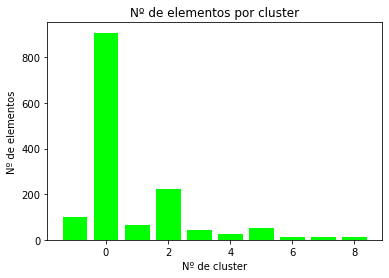
\includegraphics[width=74mm]{imagenes/c1_dbscan_cluster_01}
\end{figure}

Vemos que se han formado diez clústers, siendo el clúster con identificador $-1$  aquel compuesto por todos los datos que no encajaban en ningúno de los otros nueve. Hay 100 datos pertenecientes a este clúster, es decir, el $6.91\%$ de los datos no se clasifica correctamente. El clúster cero tiene más instancias que el resto, un total de 908, seguido del clúster dos, que tiene 221. Los clústers 1 y 3 tienen 65 y 51 instancias respectivamente, y el resto de clústers no superan las 41 instancias.

Los valores de las métricas para este modelo son:

\begin{center}
\begin{tabular}{|c|c|}
\hline
\multicolumn{1}{|c|}{\textbf{Silhouette}} & \textbf{Calinski-Harabasz}\\ \hline
  0.4869805568764864  & 165.50098317272966  \\ \hline
\end{tabular}
\end{center}

Los centroides de los diferentes clusters son:

\begin{figure}[H]
  \centering
  \caption{Centroides}
  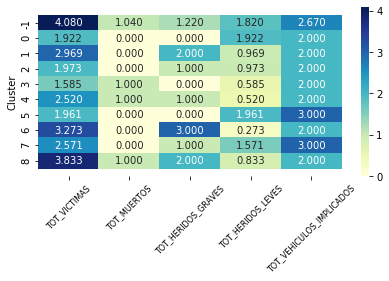
\includegraphics[width=130mm]{imagenes/c1_dbscan_centroides}
\end{figure}

El clúster 0 tiene como centro un accidente con 2 vehículos implicados, en el que 1.922 personas han sido heridos leves, pero sin muertos ni heridos graves. Este clúster es aquel con mayor número de instancias, conteniendo el $62.71\%$ de instancias. Este clúster por tanto estará formado mayoritariamente por accidentes sin heridos graves ni muertos, y con dos heridos leves.

El clúster 1 tiene como centro un accidente con 2.969 víctimas, dos heridos graves y 0.969 heridos leves, sin muertos. Dos vehículos se han visto involucrados. Este clúster estará formado mayoritariamente por accidentes con dos heridos graves y un herido leve.

El clúster 2 tiene como centro un accidente con 1.973 víctima, un herido grave y 0.973 heridos leves, y dos vehículos implicados. Es el segundo clúster con mayor número de accidentes. Este clúster estará formado mayoritariamente por accidentes con un heridos graves y un herido leve.

El clúster 3 tiene como centro un accidente con 1.585 víctimas, de las cuales una es un muerto y 0.585, heridos leves. Hubo dos vehículos implicados. Este clúster estará formado principalmente por accidentes con un muerto y entre cero y un herido leve.

El clúster 4 tiene como centro un accidente con dos vehículos implicados, que tiene como resultado 2.52 víctimas, un muerto, un herido grave y 0.52 heridos leves. Podemos deducir que este clúster lo formarán principalmente accidentes con un muerto, un herido grave y entre cero y un herido leve.

El clúster 5 tiene como centro un accidente con 1.961 víctimas, todas ellas heridos leves. Hubo tres vehículos implicados. Por tanto, este clúster lo formarán accidentes sin heridos graves ni muertos, y mayoritariamente dos heridos leves.

El clúster 6 tiene como centro un accidente con 3.273 víctimas, tres heridas gravemente y 0.273 heridos leves. Hubo dos vehículos implicados en este accidente. Es el clúster con menos instancias, sólo 11. Este clúster lo formarán principalmente los accidentes con mayor número de heridos graves, tres de media, y sin muertos ni heridos leves, ya que el número de heridos leves es más cercano a cero que a uno.

El clúster 7 tiene como centro un accidente con 2.571 víctimas, un herido grave y el resto heridos leves. Hubo tres vehículos implicados. Formarán este clúster los accidentes con un herido grave y entre uno y dos heridos leves.

El clúster 8 tiene como centro un accidente con un muerto, dos heridos graves y 0.833 heridos leves. Hubo dos vehículos implicados. Es el segundo clúster con menor número de instancias. Este clúster estará formado por tanto por accidentes con un muerto, dos heridos graves y principalmente un herido leve.

El centro del clúster $-1$ no aporta mucha información, dado que está compuesto por todos aquellos datos que no encajan con el resto de clúster, por lo tanto hay una gran variabilidad entre los atributos de los accidentes asignados a este clúster.

Para visualizar los centroides se usó el siguiente codigo:

\begin{lstlisting}
datos_cen = caso1.copy()
datos_cen.columns = atributos
datos_cen['Cluster'] = results.labels_

centroids = datos_cen.groupby('Cluster').mean()
visualize_centroids_dbscan(centroids, np.array(caso1), atributos)
\end{lstlisting}

Donde la función \texttt{visualize\_centroids\_dbscan} es análoga a la función \texttt{visualize\_centroids}, pero no aplica \texttt{denorm}, ya que los centroides no se le pasan normalizados.

Como con K-Mean, utilizé \texttt{pairplot} con la esperanza de ver diferencias entre los distintos clústers, pero sólo se aprecian las distribuciones de los atributos \texttt{TOT\_VICTIMAS} y \texttt{TOT\_HERIDOS\_GRAVES} en los clústers cero y dos, los dos clústers con más accidentes. Vemos también que hay accidentes con cinco y seis vehículos implicados y que estos tienen un número de heridos y muertos menor que alguno de los accidentes con sólo dos vehículos.

\begin{figure}[H]
  \centering
  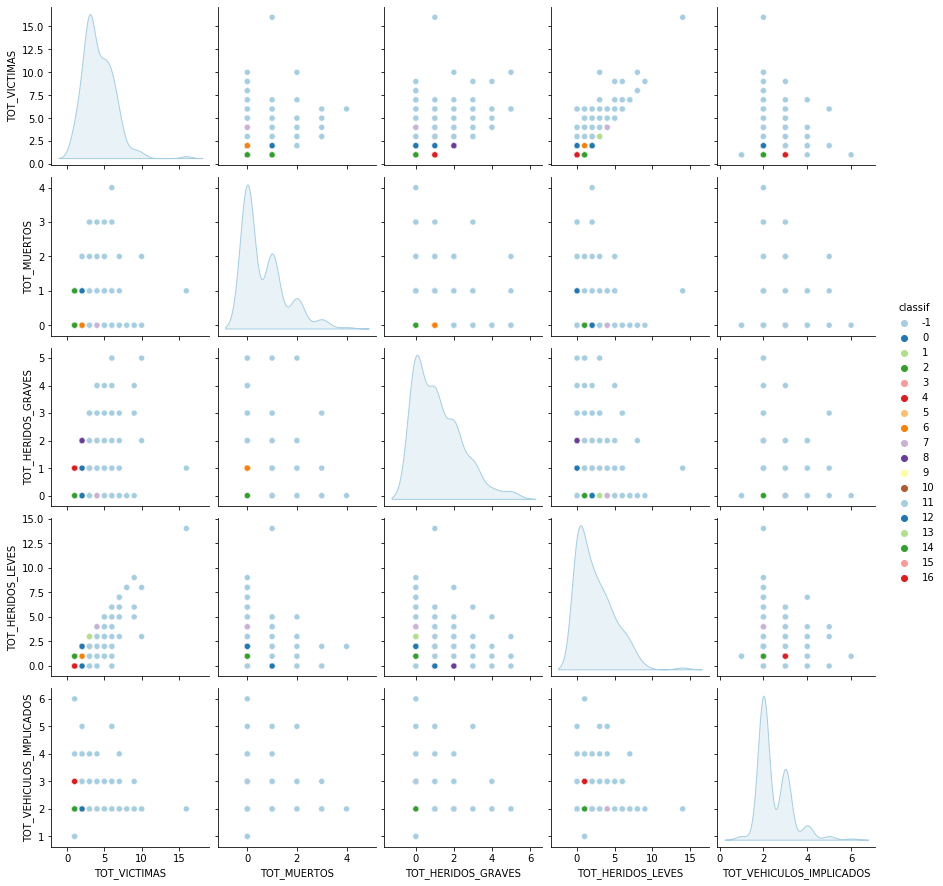
\includegraphics[width=153mm]{imagenes/c1_dbscan_pairplot}
\end{figure}

Representamos pues diagramas de cajas para poder ver mejor la variabilidad de los diferentes atributos en cada clúster y diferenciarlos así.

\begin{figure}[H]
  \centering
  \caption{Diagramas de cajas}
  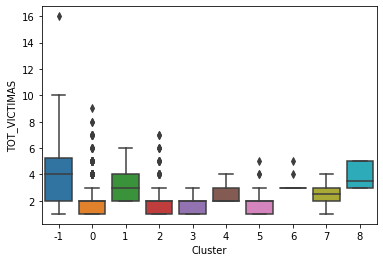
\includegraphics[width=87mm]{imagenes/c1_dbscan_vic}
  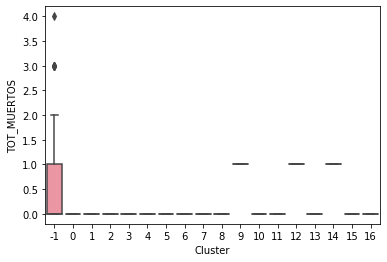
\includegraphics[width=87mm]{imagenes/c1_dbscan_muertos}
    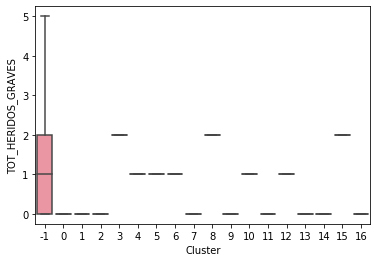
\includegraphics[width=87mm]{imagenes/c1_dbscan_hg}
  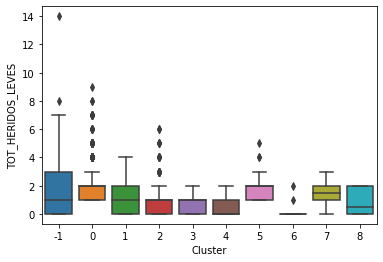
\includegraphics[width=87mm]{imagenes/c1_dbscan_hl}
  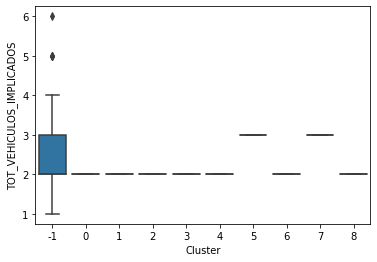
\includegraphics[width=87mm]{imagenes/c1_dbscan_vi}
\end{figure}

El clúster $-1$ es aquel con más variabilidad en todos los atributos por estar compuesto por todos aquellos accidentes que no encajaban en el resto de clústers, es por eso que sus atributos tienen más variabilidad que en el resto de clústers.

\newpage
En la siguiente tabla mostramos el rango de valores más representativo de cada cluster:

\begin{center}
\begin{tabular}{|c|c|c|c|c|c|}
\hline
\multicolumn{1}{|c|}{\textbf{Nº del clúster}} & \textbf{Víctimas} & \textbf{Muertos} & \textbf{Heridos graves} & \textbf{Heridos leves} & \textbf{Vehículos implicados}\\ \hline
  0  & 1-3 & 0 & 0 & 1-3 & 2 \\ \hline
  1  & 2-6 & 0 & 2 & 0-4 & 2 \\ \hline
  2  & 1-3 & 0 & 1 & 0-2 & 2 \\ \hline
  3  & 1-3 & 1 & 0 & 0-2 & 2 \\ \hline
  4  & 2-4 & 1 & 1 & 0-2 & 2 \\ \hline
  5  & 1-3 & 0 & 0 & 1-3 & 3 \\ \hline
  6  & 3   & 0 & 3 & 0   & 2 \\ \hline
  7  & 1-4 & 0 & 1 & 0-3 & 3 \\ \hline
  8  & 3-5 & 1 & 2 & 0-2 & 2 \\ \hline
\end{tabular}
\end{center}

El clúster 0 está formado por accidentes sin heridos graves ni muertos, donde la mayoría de ellos tienen entre 1 y 3 heridos leves. En ellos hay dos vehículos implicados.

El clúster 1 está formado por accidentes con dos vehículos implicados, sin muertos, dos heridos graves y entre 0 y 4 heridos leves, estando la mediana en un herido leve.

EL clúster 2 está compuesto poraccidentes sin muertos, un herido grave y entre 0 y 2 heridos leves. Se vieron involucrados dos vehículos.

El clúster 3 está compuesto por accidentes con dos vehículos implicados, un muerto, entre 0 y 2 heridos leves y sin heridos graves.

El clúster 4 está compuesto por accidentes con dos vehículos implicados, un muerto, un herido grave y  entre 0 y 2 heridos leves.

El clúster 5 está formado por accidentes con entre 1 y 3 víctimas, todas ellas heridos leves. Hubo tres vehículos implicados. La diferencia de este clúster con el clúster cero es el número de vehículos implicados.

El clúster 6 está compuesto por accidentes con 3 víctimas, todas ellas heridos graves. Hubo dos vehículos implicados.

El clúster 7 está compuesto por accidentes con entre 1 y 4 víctimas, un herido grave y entre 0 y 3 heridos leves, y con tres vehículos implicados.

El clúster 8 está formado por accidentes con un muerto, dos heridos graves y entre 0 y dos leves. Hubo dos vehículos implicados.

Vemos que los atributos \texttt{TOT\_MUERTOS}, \texttt{TOT\_HERIDOS\_GRAVES} y \texttt{TOT\_VEHICULOS\_IMPLICADOS} apenas tienen variabilidad dentro de cada clúster.

\subsubsection{Comparación de los algoritmos}

Los resultados de los algoritmos considerados son:

\begin{center}
\begin{tabular}{|c|c|c|c|}
\hline
  \multicolumn{1}{|c|}{\textbf{Algoritmo}} & \textbf{Silhouette} & \textbf{Calinski-Harabasz} &  \textbf{Nº de clústers}\\ \hline
  K-Means & 0.531569055229591   & 683.2263367508311  & 5  \\ \hline
  DBSCAN  & 0.4869805568764864  & 165.50098317272966 & 10 \\ \hline
\end{tabular}
\end{center}

Vemos que el algoritmo K-Means obtiene un valor de la métrica Calinski-Harabasz más de cuatro veces superior del valor que obtiene DBSCAN con esa misma métrica. También obtiene un mayor valor en la métrica Silhouettte. Por tanto, podríamos decir que el algoritmo Kmeans tiene un mejor desempeño que el DBSCAN en este caso.

El algoritmo DBSCAN divide los accidentes en más clústers que el Kmeans, y la variabilidad de los atributos en cada clústers es menor. Además la distribución de clústers es menos homogenea, habiendo cinco clústers con menos de 50 instancias.

El algoritmo Kmeans tiene por tanto mejor comportamiento que el DBSCAN, consiguiendo mejor valor en la métrica Calinski-Harabasz, y consigue agrupar los accidentes en cinco clusters claramente diferenciados, aumentando ligeramente la variabilidad de cada atributo en la cluster.

\subsubsection{Interpretación de la segmentación}

En la mayoría de accidentes hay dos vehículos implicados, por lo que el atributo \texttt{TOT\_VEHICULOS\_IMPLICADOS} no aporta mucha información. El atributo \texttt{TOT\_VICTIMAS} tampoco es muy relevante, puesto que puede calcularse a partir de \texttt{TOT\_MUERTOS}, \texttt{TOT\_HERIDOS\_GRAVES} y \texttt{TOT\_HERIDOS\_LEVES}. El atributo \texttt{TOT\_MUERTOS} sirve para diferenciar uno o tres clúster en cada uno de los modelos considerados del resto, y el resto de clústers se diferencian entre sí por los atributos \texttt{TOT\_HERIDOS\_GRAVES} y \texttt{TOT\_HERIDOS\_LEVES}, por lo que estos son los atributos dos más relevantes para el agrupamiento.

\newpage
\subsection{Caso 2: Fin de semana con densidad de circulación densa}

Nos preguntamos si durante los fines de semana hay un mayor número de víctimas que el resto de la semana, por lo que visualizamos el diagrama de cajas del atributo \texttt{TOT\_VICTIMAS} respecto al día de la semana.

\begin{figure}[H]
  \centering
  \caption{Diagramas de cajas}
  \includegraphics[width=87mm]{imagenes/c2_selec_atr}
\end{figure}

Obtenemos que efectivamente la variabilidad de este atributo es mayor en el fin de semana que en el resto de días. Además vemos no hay en la base de datos un número de accidentes significativo mayor cualquiera de estos días, es decir, que el número de accidentes cada día es más o menos homogeneo. Por estos motivos decidimos elegir como nuestro segundo caso los accidentes ocurridos los viernes, sábados o domingos. Además, elegí aquellos accidentes en los que la densidad de circulación es ``DENSA'', que representarán los días en los que mucha gente se desplace para disfrutar del fin de semana, como festividades.

\subsubsection{K-means}

Para elegir el mejor valor para el número de clústers que considera el algoritmo K-means, ejecuté el algoritmo con un número de clústers comprendido entre 2 y 14. Los resultados de las métricas son:

\begin{center}
\begin{tabular}{|c|c|c|}
\hline
\multicolumn{1}{|c|}{\textbf{Nº de clústers}}& \textbf{Silhouette} & \textbf{Calinski-Harabasz}\\ \hline
  2  & 0.5370884902834917 & 680.6474578600636  \\ \hline
  3  & 0.5022253639905714 & 691.2087946486065  \\ \hline
  4  & 0.5253455054070136 & 731.3590806547992  \\ \hline
  5  & 0.494182230718928  & 794.2278720981091  \\ \hline
  6  & 0.5384826599151725 & 904.0949725499044  \\ \hline
  7  & 0.601310808513732  & 925.9700253681594  \\ \hline
  8  & 0.622859268196415  & 942.1012174830314  \\ \hline
  9  & 0.7013609213343277 & 963.5793862878563  \\ \hline
 10  & 0.7221502954295131 & 954.6141788919715  \\ \hline
 11  & 0.7266476702162132 & 964.5578901852715  \\ \hline
 12  & 0.7385815169799497 & 996.4201247190041  \\ \hline
 13  & 0.7445925945766767 & 1032.2367917798642 \\ \hline
 14  & 0.7557938837992468 & 1058.1110463372995 \\ \hline
\end{tabular}
\end{center}

Para facilitar la comprensión de la tabla, visualizamos la información que contiene en las siguientes gráficas:

\begin{figure}[H]
  \centering
  \caption{Gráficas con el valor de las métricas en función del número de clústers}
  \includegraphics[width=87mm]{imagenes/c2_kmeans_sil}
  \includegraphics[width=87mm]{imagenes/c2_kmeans_cal}
\end{figure}

Vemos que ambas métricas aumentan cuanto mayor es el número de clústers considerados, pero un número de clústers muy alto puede tener con resultado que el modelo esté más sobreajustado. Podemos comprobar esto en las siguientes gráficas:

\begin{figure}[H]
  \centering
  \caption{Clústers}
  \includegraphics[width=57mm]{imagenes/c2_kmeans_clusters_5}
  \includegraphics[width=57mm]{imagenes/c2_kmeans_clusters}
  \includegraphics[width=57mm]{imagenes/c2_kmeans_clusters_13}
\end{figure}

Con 13 clústers hay 6 clústers con menos de 50 accidentes, con 9 clúster solo hay 2 con menos de 50 accidentes y con 5 clústers solo uno. Con ánimo de tener una métrica Calinski-Harabasz alta pero sin tener clústers con pocas instancias, que pueden ser causa del sobreajuste del modelo, utilizaremos nueve clústers.

El resultado de la segmentación es la división del conjunto de accidentes considerados en 9 conjuntos con las siguiente distribución:

\begin{figure}[H]
  \centering
  \caption{Clústers}
  \includegraphics[width=81mm]{imagenes/c2_kmeans_clusters}
\end{figure}

El clúster con más accidentes es el 2, con 415 accidentes, seguido del clúster 6, que posee 240. Los clúster con menos accidentes son el 3 con 17 y el 4 con 48.

Los valores de las métricas para este modelo son:

\begin{center}
\begin{tabular}{|c|c|}
\hline
\multicolumn{1}{|c|}{\textbf{Silhouette}} & \textbf{Calinski-Harabasz}\\ \hline
  0.7013609213343277 & 963.5793862878563 \\ \hline
\end{tabular}
\end{center}

Los centroides de los diferentes clusters son:

\begin{figure}[H]
  \centering
  \caption{Centroides}
  \includegraphics[width=130mm]{imagenes/c2_kmeans_centroides}
\end{figure}

El clúster 0 tiene como centro un accidente con 3.244 vehículos implicados, en el que 0.993 personas han sido heridos leves y 0.007 heridos graves, pero sin muertos. Por tanto los accidentes más representativos de este clúster serán aquellos sin muertos ni heridos graves, y un herido leve.

El clúster 1 tiene como centro un accidente con 3.312 víctimas, 3.262 heridos leves y 0.050 heridos graves, sin muertos. Se han visto involucrados 2.404 vehículos. Este clúster estará formado principalmente por accidentes con tres víctimas, todas ellas heridos leves.

El clúster 2 tiene como centro un accidente con 1 víctima, herida levemente, y dos vehículos implicados. Parece que la variavilidad de accidentes de este clúster es baja, coincidiendo con su centro los accidentes que lo forman.

El clúster 3 tiene como centro un accidente con 1.941 vehículos implicados, en el que 1.294 personas han sido heridos leves, 0.588 heridos leves y un muerto. Este clúster lo formarán aquellos accidentes con muertos. La media de muertos de este clústere es uno.

El clúster 4 tiene como centro un accidente con 5.771 víctimas, 5.604 heridos leves y 0.167 heridos graves, sin muertos. Se han visto involucrados 3.125 vehículos. Este clúster se caracteriza por un alto número de heridos leves, la mayoría de los accidentes de él tendrán entre cinco y seis heridos leves.

El clúster 5 tiene como centro un accidente con 1.372 víctimas, 0.271 heridos leves y 1.101 heridos graves, sin muertos. Se han visto involucrados 1.636 vehículos. Este clúster se caracteriza por tener el mayor número de heridos graves, pero la mayoría de accidentes que lo componen no tendrán ni muertos ni heridos leves.

El clúster 6 tiene como centro un accidente con 2 víctimas, heridas levemente, sin heridos graves ni muertos. Se han visto involucrados 2.112 vehículos. Loa accidentes de este clúster no presentan una alta variabilidad con su centro excepto en el número de vehículos involucrados, que será entorno a dos en la mayoría de éstos.

El clúster 7 tiene como centro un accidente con 4.773 vehículos implicados, en el que 2.32 personas han sido heridos leves, 0.013 heridos leves y sin muertos. Los accidentes de este clúster son aquellos con más vehículos involucrados, estando la media cercana a cinco vehículos. En éstos no suele haber ni heridos ni muertos y hay entre dos y tres heridos leves de media.

El clúster 8 tiene como centro un accidente con una víctimas, herida levemente, sin heridos graves ni muertos y un sólo vehículo implicado. Los accidentes de este clúster parecen no tener ninguna variabilidad respecto a su centro.

Utilizamos la función \texttt{pairplot} para ver las diferencias entre los distintos clústers:

\begin{figure}[H]
  \centering
  \includegraphics[width=180mm]{imagenes/c2_kmeans_pairplot}
\end{figure}

Los atributos \texttt{TOT\_VICTIMAS} y \texttt{TOT\_VEHICULOS\_IMPLICADOS} son aquellos que más ayudan a discernir los diferentes clústers, ya que vemos que las distribuciones de estos atributos son muy dispares en cada uno de los clústers. Los atributos \texttt{TOT\_HERIDOS\_LEVES} y \texttt{TOT\_HERIDOS\_GRAVES} diferencia los clústers 5, 0 y 7 y 1. El atributo \texttt{TOT\_MUERTOS} no aporta tanta información, ya que su media vale 0 en la mayoría de los clústers.

\newpage
Visualizamos a continuación los diagramas de cajas de los diferentes atributos en cada clúster.

\begin{figure}[H]
  \centering
  \caption{Diagramas de cajas}
  \includegraphics[width=87mm]{imagenes/c2_kmeans_vic}
  \includegraphics[width=87mm]{imagenes/c2_kmeans_muertos}
    \includegraphics[width=87mm]{imagenes/c2_kmeans_hg}
  \includegraphics[width=87mm]{imagenes/c2_kmeans_hl}
  \includegraphics[width=87mm]{imagenes/c2_kmeans_vi}
\end{figure}

\newpage
En la siguiente tabla mostramos el rango de valores más representativo de cada cluster:

\begin{center}
\begin{tabular}{|c|c|c|c|c|c|}
\hline
\multicolumn{1}{|c|}{\textbf{Nº del clúster}} & \textbf{Víctimas} & \textbf{Muertos} & \textbf{Heridos graves} & \textbf{Heridos leves} & \textbf{Vehículos implicados}\\ \hline
  0  & 1   & 0 & 0   & 1   & 3   \\ \hline
  1  & 3-4 & 0 & 0   & 3-4 & 1-4 \\ \hline
  2  & 1   & 0 & 0   & 1   & 2   \\ \hline
  3  & 1-6 & 1 & 0-2 & 0-4 & 1-3 \\ \hline
  4  & 5-7 & 0 & 0   & 4-7 & 1-6 \\ \hline
  5  & 1-3 & 0 & 1   & 0   & 1-3 \\ \hline
  6  & 2   & 0 & 0   & 2   & 2   \\ \hline
  7  & 1-4 & 0 & 0   & 1-4 & 4-6 \\ \hline
  8  & 1   & 0 & 0   & 1   & 1   \\ \hline
\end{tabular}
\end{center}

El clúster $0$ está compuesto por accidentes con 3 vehículos implicados sin muertos ni heridos graves y un herido leve.

El clúster $1$ está formado por accidentes con entre tres y cuatro heridos leves, sin muertos o heridos leves. Se vieron implicados entre uno y cuatro vehículos.

El clúster $2$ está compuesto por accidentes sin muertos ni heridos graves y un herido leve. Se diferencia del clúster 0 por tener 2 vehículos implicados en lugar de tres. Es aquel con más muestras.

El clúster $3$ es el único cluste en cuyos accidentes hay muertos. Hay un muerto concretamente. También hay entre cero y dos heridos graves y entre cero y cuatro leves. Se vieron involucrados entre uno y tres vehículos. Es el clúster con menos muestras.

El clúster $4$ se compone de accidentes con entre cuatro y siete víctimas, todas ellas heridos leves. Puede haber entre uno y seis vehículos implicados.

El clúster $5$ se compone de accidentes con entre uno y tres vehículos implicados y entre una y tres víctimas.

El clúster $6$ se compone de accidentes con dos víctimas, todos ellos heridos leves, y dos vehículos implicados. Es el segundo clúster con mayor número de muestras.

El clúster $7$ se compone de accidentes con entre una y cuatro víctimas, todas ellas heridos leves. Puede haber entre cuatro y seis vehículos implicados.

El clúster $8$ está compuesto por accidentes sin muertos ni heridos graves y un herido leve. Se diferencia del clúster 0 y 2 por tener un solo vehículo implicado en lugar de dos o tres. Tiene menos muestras que el clúster dos, pero más que el cero.

En la mayoría de accidentes no hay muertos, por lo que el atributo \texttt{TOT\_MUERTOS} sólo ayuda a diferenciar el clúster 3, compuesto por 17 instancias, del resto. El atributo \texttt{TOT\_HERIDOS\_GRAVES} sólo difiere de cero en los clúster 3 y 5. El resto de clústers se diferencian entre sí por los atributos \texttt{TOT\_HERIDOS\_LEVES} y \texttt{TOT\_VEHICULOS\_IMPLICADOS}, por lo que estos son los atributos dos más relevantes para el agrupamiento.

\subsubsection{DBSCAN}

Al igual que en el caso 1, estimamos el valor del parámetro \textit{epsilon}, la distancia a la que consideramos que dos puntos son directamente alcanzables. El valor de \textit{min\_samples} considerado sigue siendo diez. Ejecuté el algoritmo con diez valores de \textit{epsilon} equidistantes entre 0.02 y 0.2, ambos incluidos. Los resultados de las métricas son:

\begin{center}
\begin{tabular}{|c|c|c|}
\hline
\multicolumn{1}{|c|}{\textbf{Epsilon}}& \textbf{Silhouette} & \textbf{Calinski-Harabasz}\\ \hline
  0.02  & 0.82892254556956    & 116.97236922937577  \\ \hline
  0.04  & 0.8289225455695599  & 116.97236922937577  \\ \hline
  0.06  & 0.8289225455695599  & 116.97236922937577  \\ \hline
  0.08  & 0.82892254556956    & 116.97236922937577  \\ \hline
  0.1   & 0.82892254556956    & 116.97236922937577  \\ \hline
  0.12  & 0.8289225455695599  & 116.97236922937577  \\ \hline
  0.14  & 0.4536119566421056  & 220.24625024938823  \\ \hline
  0.16  & 0.4045951263790732  & 200.4202941262233   \\ \hline
  0.18  & 0.4045951263790732  & 200.4202941262233   \\ \hline
  0.2   & 0.40701069566142584 & 172.58676418042137  \\ \hline
\end{tabular}
\end{center}

Para facilitar la comprensión de la tabla, visualizamos la información que contiene en las siguientes gráficas:

\begin{figure}[H]
  \centering
  \caption{Gráficas con el valor de las métricas en función del número de clústers}
  \includegraphics[width=73mm]{imagenes/c2_dbscan_sil}
  \includegraphics[width=73mm]{imagenes/c2_dbscan_cal}
\end{figure}

Seleccioné el valor de \textit{epsilon} = 0.14 porque es en el que se maximiza la métrica Calinski-Harabasz. La métrica Silhouette no utiliza todas las muestras para su cálculo y depende entonces de las muestras seleccionadas, por lo que decidí anteponer la maximización de la métrica Calinski-Harabasz a la de ésta. Los clústers formados quedan así:

\begin{figure}[H]
  \centering
  \caption{Clústers}
  \includegraphics[width=87mm]{imagenes/c2_dbscan_clusters}
\end{figure}

Vemos que se han formado 9 cluster, siendo el clúster con identificador $-1$ aquel compuesto por todos los datos que no encajaban en ningúno de los otros 8. Hay 61 datos pertenecientes a este clúster, es decir, el $4.41\%$ de los datos no se clasifica correctamente. El clúster con más instancias es el 0, que cuenta con 740, seguido del clúster 3, con 273. Los clústers que superan las 100 instancias son el clúster 0, el 3 y el 5. El clúster 2 tiene 98, y el resto menos de 65. 

Los valores de las métricas para este modelo son:

\begin{center}
\begin{tabular}{|c|c|}
\hline
\multicolumn{1}{|c|}{\textbf{Silhouette}} & \textbf{Calinski-Harabasz}\\ \hline
  0.4536119566421056  & 220.24625024938823  \\ \hline
\end{tabular}
\end{center}

Los centroides de los diferentes clusters son:

\begin{figure}[H]
  \centering
  \caption{Centroides}
  \includegraphics[width=130mm]{imagenes/c2_dbscan_centroides}
\end{figure}

El clúster 0 tiene como centro un accidente con 2.012 vehículos implicados, en el que una persona ha sido herida levemente, pero sin muertos ni heridos graves.

El clúster 1 tiene como centro un accidente con dos víctimas, una herida leve y otra herida grave, sin muertos. Se han visto involucrados 1.947 vehículos.

El clúster 2 tiene como centro un accidente con 1 víctima, herida gravemente, y 1.596 vehículos implicados.

El clúster 3 tiene como centro un accidente con dos víctimas, ambas heridos leves. Hubo 2.370 vehículos implicados.

El clúster 4 tiene como centro un accidente con 6 víctimas, todas ellas heridos leves, y 2.824 vehículos implicados.

El clúster 5 tiene como centro un accidente con 3 víctimas, todas ellas heridos leves, y 2.726 vehículos implicados.

El clúster 6 tiene como centro un accidente con 2.886 vehículos implicados en que que 4 personas resultaron heridas levemente.

El clúster 7 tiene como centro un accidente con 5 víctimas, las cinco heridas leves. Hubo tres vehículos implicados.

Los accidentes que componen los clústers representativos parecen no tener ninguna variabilidad respecto a su centro en todos los atributos a excepción del número de vehículos implicados, por tanto los accidentes que los forman son aquellos que tienen exáctamente el mismo valor en todos sus atributos a excepción del número de vehículos implicados que el centro.

Vemos que el atributo \texttt{TOT\_MUERTOS} tiene media cero en todos los clústers, y sólo dos de ellos tienen de media el atributo \texttt{TOT\_HERIDOS\_GRAVES} distinto de cero. Los atributos que más varían entre los clústers son \texttt{TOT\_HERIDOS\_LEVES} y \texttt{TOT\_VEHICULOS\_IMPLICADOS}.

Como con K-Mean, utilizé \texttt{pairplot} con la esperanza de ver diferencias entre los distintos clústers, pero los resultados no son los esperados y sólo podemos ver la distribución del atributo \texttt{TOT\_VEHICULOS\_IMPLICADOS} en los diferentes clústers, que, como veremos a continuación en el diagrama de cajas, es el único atributo con variabilidad en los clústers.

\begin{figure}[H]
  \centering
  \includegraphics[width=180mm]{imagenes/c2_dbscan_pairplot}
\end{figure}

Representamos pues diagramas de cajas para poder ver mejor la variabilidad de los diferentes atributos en cada clúster y diferenciarlos así.

\begin{figure}[H]
  \centering
  \caption{Diagramas de cajas}
  \includegraphics[width=87mm]{imagenes/c2_dbscan_vic}
  \includegraphics[width=87mm]{imagenes/c2_dbscan_muertos}
    \includegraphics[width=87mm]{imagenes/c2_dbscan_hg}
  \includegraphics[width=87mm]{imagenes/c2_dbscan_hl}
  \includegraphics[width=87mm]{imagenes/c2_dbscan_vi}
\end{figure}

El clúster $-1$ es aquel con más variabilidad en todos los atributos por estar compuesto por todos aquellos accidentes que no encajaban en el resto de clústers. El resto de clústers tienen poca variabilidad en la mayoría de los atributos, a excepción del \texttt{TOT\_VEHICULOS\_IMPLICADOS}. El atributo \texttt{TOT\_MUERTOS} no aporta información en el agrupamiento, ya que ninguno de los clústers formados contiene contiene accidentes con muertos, todos estos accidentes son colocados en el clúster $-1$, junto con el resto de accidentes que no es capaz de clasificar correctamente.

\newpage
En la siguiente tabla mostramos el rango de valores más representativo de cada clúster:

\begin{center}
\begin{tabular}{|c|c|c|c|c|c|}
\hline
\multicolumn{1}{|c|}{\textbf{Nº del clúster}} & \textbf{Víctimas} & \textbf{Muertos} & \textbf{Heridos graves} & \textbf{Heridos leves} & \textbf{Vehículos implicados}\\ \hline
  0  & 1 & 0 & 0 & 1 & 2   \\ \hline
  1  & 2 & 0 & 1 & 1 & 1-2 \\ \hline
  2  & 1 & 0 & 1 & 0 & 1-3 \\ \hline
  3  & 2 & 0 & 0 & 2 & 1-4 \\ \hline
  4  & 6 & 0 & 0 & 6 & 1-4 \\ \hline
  5  & 3 & 0 & 0 & 3 & 1-4 \\ \hline
  6  & 4 & 0 & 0 & 4 & 2-5 \\ \hline
  7  & 5 & 0 & 0 & 5 & 2-5 \\ \hline
\end{tabular}
\end{center}

Como el único atributo con variabilidad es \texttt{TOT\_VEHICULOS\_IMPLICADOS}, lo único que diferencia a cada instancia de un clúster del centro de éste es el número de vehículos involucrados en dicho accidente. Este atributo junto con \texttt{TOT\_HERIDOS\_LEVES} es el que más ayuda a la diferenciacion de los distintos clústers entre sí.

\subsubsection{Comparación de los algoritmos}

Los resultados de los algoritmos considerados son:

\begin{center}
\begin{tabular}{|c|c|c|c|}
\hline
  \multicolumn{1}{|c|}{\textbf{Algoritmo}} & \textbf{Silhouette} & \textbf{Calinski-Harabasz} &  \textbf{Nº de clústers}\\ \hline
 Kmeans &  0.7013609213343277  & 963.5793862878563  & 9 \\ \hline
 DBSCAN &  0.4536119566421056  & 220.24625024938823 & 9 \\ \hline
\end{tabular}
\end{center}

Aunque ambos algoritmos crean el mismo número de clústers, el algoritmo K-means tiene un mejor desempeño que el DBSCAN. El K-means consigue clústers cuyos atributos tienen mayor variabilidad, como nos ocurría en el caso 1, y las instancias están divididas en los clústers de manera más homogenea, mientras que con DBSCAN hay mayor diferencia entre el número de instancias en el clúster ``más poblado'', el clúster 0, y en el resto.

\subsubsection{Interpretación de la segmentación}

Con los dos algoritmos considerados los atributos que mejor diferencian los distintos clústers son \texttt{TOT\_VEHICULOS\_IMPLICADOS} y \texttt{TOT\_HERIDOS\_LEVES}. No hay muchos accidentes en este caso con muertos, por lo que el atributo \texttt{TOT\_MUERTOS} no ayuda mucho a diferencias los distintos clústers. De hecho, el algortimo DBSCAN descarta los casos con muertos y los clasifica en el clúster $-1$. Como comentamos anteriormente, el atributo \texttt{TOT\_VICTIMAS} puede deducirse de otros atributos considerados, por lo que podríamos prescindir de él. En ambos casos, el atributo \texttt{TOT\_HERIDOS\_LEVES} sólo ayuda a diferenciar dos clúster de los otros siete.

\newpage

\subsection{Caso 3: Entre semana con densidad de circulación densa}

Añadimos el caso de estudio ``Entre semana con densidad de circulación densa'' para contrastar las características de los accidentes ocurridos bajo estas casuísticas con las de los accidentes del caso 2 y ver las diferencias entre ambos.

\subsubsection{K-means}

Para elegir el mejor valor para el número de clústers que considera el algoritmo K-means, ejecuté el algoritmo con un número de clústers comprendido entre 2 y 14. Los resultados de las métricas son:

\begin{center}
\begin{tabular}{|c|c|c|}
\hline
\multicolumn{1}{|c|}{\textbf{Nº de clústers}}& \textbf{Silhouette} & \textbf{Calinski-Harabasz}\\ \hline
  2  & 0.7901017312445583 & 3323.5016323001405 \\ \hline
  3  & 0.6905258174794837 & 3525.6287793192128 \\ \hline
  4  & 0.7165882158328284 & 3618.7158935218295 \\ \hline
  5  & 0.6997302171607823 & 3795.7422278443883 \\ \hline
  6  & 0.7081949623134676 & 4701.55145591241   \\ \hline
  7  & 0.7172739598299913 & 4917.07511849222   \\ \hline
  8  & 0.7180182979610455 & 5328.48275510556   \\ \hline
  9  & 0.7093267907202339 & 5365.78866185542   \\ \hline
 10  & 0.7196928899841787 & 5423.52585949096   \\ \hline
 11  & 0.7234741493620663 & 5615.46939478977   \\ \hline
 12  & 0.7232982041710021 & 5867.24077956305   \\ \hline
 13  & 0.7192164530386997 & 6188.01750953239   \\ \hline
 14  & 0.6974543104655523 & 6464.06705569186   \\ \hline
\end{tabular}
\end{center}

Para facilitar la comprensión de la tabla, visualizamos la información que contiene en las siguientes gráficas:

\begin{figure}[H]
  \centering
  \caption{Gráficas con el valor de las métricas en función del número de clústers}
  \includegraphics[width=87mm]{imagenes/c3_kmeans_sil}
  \includegraphics[width=87mm]{imagenes/c3_kmeans_cal}
\end{figure}

Vemos que la métrica Calinski-Harabasz aumenta cuanto mayor es el número de clústers considerados, mientras que la Silhouette sube y baja. Como no queremos un número alto de clústers con pocas instancias en la mayoría de ellos, para tomar esta decisión visualizamos las siguientes gráficas con el número de clústers 4, 8 y 12, que son picos en la métrica Silhouette:

\begin{figure}[H]
  \centering
  \caption{Distribución con 4, 8 y 12 clústers}
  \includegraphics[width=57mm]{imagenes/c3_kmeans_clusters_4}
  \includegraphics[width=57mm]{imagenes/c3_kmeans_clusters_8}
  \includegraphics[width=57mm]{imagenes/c3_kmeans_clusters_12}
\end{figure}

\vspace{-3mm}

Con 12 clústers hay 7 clústers con menos de 70 accidentes, con 8 clúster hay tres y con 4 clústers solo uno. A la vista de los resultados, decidí que hacer el análisis con cuatro clústers era más adecuado. Por tanto, la distribución de los clústers es:
\vspace{-3mm}

\begin{figure}[H]
  \centering
  \caption{Clústers}
  \includegraphics[width=65mm]{imagenes/c3_kmeans_clusters_4}
\end{figure}

\vspace{-3mm}

El clúster con más instancias es el 0, que cuenta con 1993 es decir, contiene el $76.65\%$ de los accidentes. El clúster 2, con 342 accidentes, es el sugundo mayor. El clúster uno tiene 233 instancias y el 3 tiene sólo 32, que representa el $1.23\%$ de éstas.

Los valores de las métricas para este modelo son:

\begin{center}
\begin{tabular}{|c|c|}
\hline
\multicolumn{1}{|c|}{\textbf{Silhouette}} & \textbf{Calinski-Harabasz}\\ \hline
  0.7165882158328284 & 3618.7158935218295  \\ \hline
\end{tabular}
\end{center}

Los centroides de los diferentes clusters son:

\vspace{-3mm}

\begin{figure}[H]
  \centering
  \caption{Centroides}
  \includegraphics[width=106mm]{imagenes/c3_kmeans_centroides}
\end{figure}

El clúster 0 tiene como centro un accidente con 2.155 vehículos implicados, en el que 1.256 personas han sido heridas levemente, pero sin muertos ni heridos graves. Este clúster es aquel con más instancias de los cuatro. Podemos deducir que este clúster estará formado por accidentes sin muertos ni heridos graves, y principalmente un herido leve.

El clúster 1 tiene como centro un accidente con 0.451 heridos leves, 1.094 heridos graves y 0.004 muertos. Se han visto involucrados 1.936 vehículos. Este clúster es el clúster con mayor número de heridos graves de media. Este clúster estará formado por los accidentes con heridos graves, entando la media en un herido grave. Además tienen entre cero y un herido leve.

El clúster 2 tiene como centro un accidente con 3.813 víctimas, 0.003 heridos graves y 3.81 heridos leves, y 3.07 vehículos implicados. Por tanto, este clúster es aquel con más heridos leves de media y más vehículos implicados. Estos accidentes son aquellos sin heridos graves ni muertos y principalmente cuatro heridos leves.

El clúster 3 tiene como centro un accidente con 1.094 víctimas, 1.094 muertos, 0.094 heridos graves y 0.219 heridos leves. Hubo 1.719 vehículos implicados. Este clúster es aquel con menos accidentes, representa el $1.23\%$ de los accidentes, y es el que mayor número de muertos tiene de media, de hecho, es el único donde la mayoría de accidentes tienen muertos, estando la media en un muerto. la mayoría de ellos no tendrán ni heridos leves ni graves.

Vemos que el clúster uno se diferencia del resto por su valor del atributo \texttt{TOT\_HERIDOS\_GRAVES} y el clúster tres por el \texttt{TOT\_MUERTOS}. El clúster dos se caracteriza por el mayor valor de los atributos \texttt{TOT\_HERIDOS\_LEVES} y \\\texttt{TOT\_VEHICULOS\_IMPLICADOS}.

Utilizé \texttt{pairplot} para ver diferencias entre los distintos clústers. Los resultados son:

\begin{figure}[H]
  \centering
  \includegraphics[width=148mm]{imagenes/c3_kmeans_pairplot}
\end{figure}

Vemos las diferentes dirtribuciones los atributos \texttt{TOT\_VICTIMAS}, \texttt{TOT\_HERIDOS\_LEVES} y \texttt{TOT\_VEHICULOS\_IMPLICADOS} entre los clústers cero, uno y dos. El atributo \texttt{TOT\_MUERTOS} separa los elementos del clúster uno de los del clúster 3. Podemos ver las diferencias entre el clúster uno, dos y tres por sus distribuciones de \texttt{TOT\_HERIDOS\_GRAVES}.

Representamos diagramas de cajas para poder ver mejor la variabilidad de los diferentes atributos en cada clúster y caracterizarlos así.

\begin{figure}[H]
  \centering
  \caption{Diagramas de cajas}
  \includegraphics[width=87mm]{imagenes/c3_kmeans_vic}
  \includegraphics[width=87mm]{imagenes/c3_kmeans_muertos}
  \includegraphics[width=87mm]{imagenes/c3_kmeans_hg}
  \includegraphics[width=87mm]{imagenes/c3_kmeans_hl}
  \includegraphics[width=87mm]{imagenes/c3_kmeans_vi}
\end{figure}

\newpage
En la siguiente tabla mostramos el rango de valores más representativo de cada clúster:

\begin{center}
\begin{tabular}{|c|c|c|c|c|c|}
\hline
\multicolumn{1}{|c|}{\textbf{Nº del clúster}} & \textbf{Víctimas} & \textbf{Muertos} & \textbf{Heridos graves} & \textbf{Heridos leves} & \textbf{Vehículos implicados}\\ \hline
  0  & 1-2 & 0 & 0 & 1-2 & 2   \\ \hline
  1  & 1-3 & 0 & 1 & 0-2 & 1-3 \\ \hline
  2  & 3-5 & 0 & 0 & 3-5 & 1-4 \\ \hline
  3  & 1-3 & 1 & 0 & 0   & 1-3 \\ \hline
\end{tabular}
\end{center}

El clúster 0 se compone de accidentes con dos vehículos implicados en los que de una a dos personas han salido heridas levemente. No hubo ni muertos ni heridos graves.

El clúster 1 se compone de accidentes con un herido grave y de cero a dos heridos leves donde de uno a tres vehículos se vieron implicados.

El clúster 2 está formado por instancias con entre tres y cinco víctimas, todas ellas heridos leves, resultantes del accidente de entre uno y cuatro vehículos.

El clúster 3 está formado principalmente por accidentes con un muerto y entre uno y tres vehículos implicados.

El clúster tres se caracteriza por el atributo \texttt{TOT\_MUERTOS}, ya que es el único con muertos, y el clúster uno por \texttt{TOT\_HERIDOS\_GRAVES}. Los otros dos clústers se diferencian por el \texttt{TOT\_HERIDOS\_LEVES}. Además, el clúster 2 tiene mayor variabilidad del atributo \texttt{TOT\_VEHICULOS\_IMPLICADOS}.

\subsubsection{DBSCAN}

Estimamos el valor del parámetro \textit{epsilon} ejecutando el algoritmo con diez valores de \textit{epsilon} equidistantes entre 0.02 y 0.2, ambos incluidos. Los resultados de las métricas son:

\begin{center}
\begin{tabular}{|c|c|c|}
\hline
\multicolumn{1}{|c|}{\textbf{Epsilon}}& \textbf{Silhouette} & \textbf{Calinski-Harabasz}\\ \hline
  0.02 & 0.8813554395557858 & 222.44145602974191 \\ \hline
  0.04 & 0.717645527812345  & 1230.4090960667304 \\ \hline
  0.06 & 0.7176455278123451 & 1230.4090960667304 \\ \hline
  0.08 & 0.7229551894566059 & 1387.6592433383134 \\ \hline
  0.1  & 0.7229551894566059 & 1387.6592433383134 \\ \hline
  0.12 & 0.7944150822377707 & 1286.7594060038498 \\ \hline
  0.14 & 0.7957146553352213 & 1340.657424226088  \\ \hline
  0.16 & 0.7955070215626333 & 1342.5476210406275 \\ \hline
  0.18 & 0.7955070215626336 & 1342.5476210406275 \\ \hline
  0.2  & 0.7955070215626334 & 1342.5476210406275 \\ \hline
\end{tabular}
\end{center}

Para facilitar la comprensión de la tabla, visualizamos la información que contiene en las siguientes gráficas:

\begin{figure}[H]
  \centering
  \caption{Gráficas con el valor de las métricas en función del número de clústers}
  \includegraphics[width=73mm]{imagenes/c3_dbscan_sil}
  \includegraphics[width=73mm]{imagenes/c3_dbscan_cal}
\end{figure}

Seleccioné el valor de \textit{epsilon} = 0.14 porque en él aumentan ambas métricas. Los clústers formados quedan así:

\begin{figure}[H]
  \centering
  \caption{Clústers}
  \includegraphics[width=87mm]{imagenes/c3_dbscan_clusters}
\end{figure}

Vemos que se han formado cinco cluster, siendo el clúster con identificador $-1$ aquel compuesto por todos los datos que no encajaban en ningúno de los otros cuatro. Hay 14 datos pertenecientes a este clúster, por tanto el $99.46\%$ de los datos se clasifica correctamente. El clúster con más instancias es el 0, que cuenta con 2331, seguido del clúster uno, con 211. Los otros dos clústers tienen menos de 30 instancias cada uno, entre los dos represenatan el $1.69\%$ de los accidentes considerados.

Los valores de las métricas para este modelo son:

\begin{center}
\begin{tabular}{|c|c|}
\hline
\multicolumn{1}{|c|}{\textbf{Silhouette}} & \textbf{Calinski-Harabasz}\\ \hline
  0.7957146553352213 & 1340.657424226088  \\ \hline
\end{tabular}
\end{center}

Los centroides de los diferentes clusters son:

\begin{figure}[H]
  \centering
  \caption{Centroides}
  \includegraphics[width=130mm]{imagenes/c3_dbscan_centroides}
\end{figure}

El clúster 0 tiene como centro un accidente con 2.269 vehículos implicados, en el que 1.618 personas han sido heridas levemente, pero sin muertos ni heridos graves. Loa accidentes de este clśter tendrán un mayor número de heridos leves, entre uno y dos, pero sin heridos graves ni muertos.

El clúster 1 tiene como centro un accidente con 1.37 víctimas, una herida grave y 0.37 heridos leves, sin muertos. Se han visto involucrados 1.858 vehículos. Por tanto, este clúster estará formado mayoritariamente por accidentes con un herido grave.

El clúster 2 tiene como centro un accidente con un muerto y 0.222 heridos leves. Hubo 1.704 vehículos implicados. Los accidentes de este clúster son aquellos con muertos, estando la media en un muerto.

El clúster 3 tiene como centro un accidente con 2.412 víctimas, dos heridos graves y 0.412 heridos leves, y 2.294 vehículos implicados. Los accidentes de este clúster son aquellos con mayor número de heridos graves, estando la media en dos. Además la mayoría tienen entre cero y un herido leve.

El clúster dos es el único con un valor medio de \texttt{TOT\_MUERTOS} distinto de cero. El clúster cero, que es el que más accidentes posee, es el único que tiene media nula tanto en \texttt{TOT\_MUERTOS} como en \texttt{TOT\_HERIDOS\_GRAVES}. Los clústers uno y tres se diferencian por su media de \texttt{TOT\_HERIDOS\_GRAVES}.

En el resto de casos no hablamos del clúster $-1$, no le vi sentido comentarlo ya que en él hay datos muy dispersos y no podemos sacar información del conjunto en sí, pero llama la atención la media de \texttt{TOT\_VEHICULOS\_IMPLICADOS}, que es más alta que en el resto de los otros clústers.

Como en el resto de casos, utilizé \texttt{pairplot} con el objetivo de ver diferencias entre los distintos clúster. Sólo se muestran las dirtribuciones de los atributos \texttt{TOT\_VICTIMAS}, \texttt{TOT\_HERIDOS\_GRAVES} y \texttt{TOT\_VEHICULOS\_IMPLICADOS} de los clústers cero y uno, que son los clústers con más instancias.

\begin{figure}[H]
  \centering
  \includegraphics[width=149mm]{imagenes/c3_dbscan_pairplot}
\end{figure}


Representamos diagramas de cajas para poder ver mejor la variabilidad de los diferentes atributos en cada clúster y caracterizarlos así.

\begin{figure}[H]
  \centering
  \caption{Diagramas de cajas}
  \includegraphics[width=87mm]{imagenes/c3_dbscan_vic}
  \includegraphics[width=87mm]{imagenes/c3_dbscan_muertos}
  \includegraphics[width=87mm]{imagenes/c3_dbscan_hg}
  \includegraphics[width=87mm]{imagenes/c3_dbscan_hl}
  \includegraphics[width=87mm]{imagenes/c3_dbscan_vi}
\end{figure}

\newpage
En la siguiente tabla mostramos el rango de valores más representativo de cada clúster:

\begin{center}
\begin{tabular}{|c|c|c|c|c|c|}
\hline
\multicolumn{1}{|c|}{\textbf{Nº del clúster}} & \textbf{Víctimas} & \textbf{Muertos} & \textbf{Heridos graves} & \textbf{Heridos leves} & \textbf{Vehículos implicados}\\ \hline
  0  & 1-3 & 0 & 0 & 1-3 & 1-4 \\ \hline
  1  & 1   & 0 & 1 & 0   & 1-3 \\ \hline
  2  & 1   & 1 & 0 & 0   & 1-3 \\ \hline
  3  & 2-4 & 0 & 2 & 0-2 & 1-4 \\ \hline
\end{tabular}
\end{center}

El clúster 0 se compone principalmente de accidentes con entre uno y cuatro vehículos implicados en los que de una a tres personas han salido heridas levemente. No hubo ni muertos ni heridos graves.

El clúster 1 se compone mayoritariamente de accidentes con una víctima, herida gravemente. De uno a tres vehículos se vieron implicados.

El clúster 2 está formado por accidentes con un muerto, sin heridos leves ni graves, con de uno a tre vehículos involucrados.

El clúster 3 está formado por accidentes con entre uno y cuatro vehículos implicados, con dos heridos graves y entre cero y dos heridos leves.

Vemos que los atributos \texttt{TOT\_MUERTOS} y \texttt{TOT\_HERIDOS\_GRAVES} no tienen variabilidad dentro de los clústers, son los mismos que observamos en los centroides. El atributo \texttt{TOT\_VEHICULOS\_IMPLICADOS} es aquel con mayor variabilidad, seguido del atributo \texttt{TOT\_HERIDOS\_LEVES}, que principalmente presenta variabilidad en los clústers cero y tres.

\subsubsection{Comparación de los algoritmos}

Los resultados de los algoritmos considerados son:

\begin{center}
\begin{tabular}{|c|c|c|c|}
\hline
  \multicolumn{1}{|c|}{\textbf{Algoritmo}} & \textbf{Silhouette} & \textbf{Calinski-Harabasz} &  \textbf{Nº de clústers}\\ \hline
 Kmeans & 0.7165882158328284 & 3618.7158935218295 & 4 \\ \hline
 DBSCAN & 0.7957146553352213 & 1340.657424226088  & 5 \\ \hline
\end{tabular}
\end{center}

Aunque ambos algoritmos crean el mismo número de clústers ``representativos'', el algoritmo K-means consigue un mayor valor de la métrica Calinski-Harabasz, mientras que el DBSCAN tiene un mayor valor de la métrica Silhouette. La variabilidad de los atributos en los clústers formados por ambos algoritmos es similar. Respecto a la distribución de los clústers, ambos obtienen un clúster con muchos más datos que el resto. El algoritmo Kmeans crea un clúster con menos de 50 instancias y el DBSCAN dos, sin contar el clúster $-1$, que es conveniente que tenga pocos datos.

\subsubsection{Interpretación de la segmentación}

Con los dos algoritmos hay un clúster más grande que el resto, que es aquel sin heridos graves ni muertos, y de uno a tres heridos leves. Por tanto vemos que en este caso de uso no suele haber accidentes muy graves. Los clústers con muertos tienen menos de 35 instancias. También hay entorno a 230 accidentes con heridos graves y sin muertos. Por tanto el atributo \texttt{TOT\_MUERTOS} caracteriza a uno de los clústers y el atributo \texttt{TOT\_HERIDOS\_GRAVES} diferencia de uno a dos de los clústers creados de los demás.

\newpage
\subsection{Comparación de los casos de estudio 2 y 3}

Comparamos los accidentes producidos de viernes a domingo (caso 2) con los accidentes producidos de lunes a jueves (caso 3).

Hay 2600 accidentes producidos de lunes a jueves mientras que el otro caso está compuesto por poco más de la mitad de accidentes, un total de 1383 accidentes. Por tanto, se producen más accidentes de lunes a jueves que el resto de días.

Vemos que en el caso dos se han formado más clústers que en el caso tres, por lo que los accidentes ocurridos de viernes a domingo parecen más variados que los ocurridos durante el resto de días.

Respecto a las víctimas de los accidentes, la proporción de accidentes con un muerto en ambos casos es muy parecida, entorno a un $1.22\%$, sin embargo, los accidentes producidos de viernes a domingo a parte del muerto hubo más heridos en dicho accidente, entre cero y dos heridos graves y entre cero y cuatro heridos leves, mientras que en el otro caso la única víctima en el accidente fue el fallecido. En ambos casos hay entre uno y tres vehículos implicados en estos accidentes. Por tanto observamos que los accidentes producidos en fin de semana con muertos tiene un mayor número de víctimas que el resto de días.

También observamos que los accidentes del caso 2 tienen un mayor número de heridos leves que los del caso 3. Si miramos el boxplot del clúster 4 formado con el algoritmo KMeans, este clúster tiene de 5 a 7 víctimas, todas ellas heridos leves. Lo mismo ocurre con el clúster 4 formado con DBSCAN, que tiene seis heridos leves. Sin embargo, en los accidentes ocurridos de lunes a jueves no hay más de 5 heridos leves. Vemos que el atributo heridos leves tiene mayor variabilidad entre los clústers del caso 2 que en el caso 3. Por consiguiente, el total de víctimas en la mayoría de los accidentes del caso dos se mueve entre una y siete, mientras que las del caso tres se mueve entre una y cinco. Además, como vimos en el boxplot que nos llevó a considerar elegir este caso de estudio, como en los clústers más poblados el número de víctimas es menor, si nos fijamos en los datos en su conjunto vemos que la mayoría de accidentes del caso tres el número de heridos es uno, mientras en el caso dos, el número de heridos está entre uno y tres.

Otra de las diferencias entre los casos es el número de coches implicados. En los accidentes producidos de viernes a domingo este atributo tiene una mayor variabilidad, habiendo clústers con hasta seis vehículos implicados, mientras que en el otro caso no hay más de cuatro vehículos implicados en estos accidentes.

En ambos casos el accidente más común es aquel sin muertos ni heridos graves, y de uno a dos heridos leves y dos vehículos implicados. Este accidente, que corresponde al clúster cero del caso tres formado por el algoritmo K-means, se puede equiparar al clúster dos y seis del caso dos formado con el mis mo algoritmo. En el caso tres, estos accidentes forman el $76.65\%$ de la muestra, mientras que en el caso dos forman el $47.36\%$. 

\newpage
\section{Contenido adicional}

En esta sección analizaremos otros atributos no contemplados en el clústering para ver qué factores intervinieron en aquellos accidentes de los clústers conseguidos con el algoritmo K-means con mayor número de víctimas.

\subsection{Caso 1}

Estudiamos los accidentes de los clústers uno, dos y tres, que son aquellos con mayor número de heridos graves, heridos leves y muertos, respectivamente. 

Primero me planteé si la severidad de estos accidentes puede deberse a poca visibilidad en la carretera, por lo que comparamos el porcentaje de accidentes con diversas condiciones de luminosidad posibles registradas en estos tres clústers. Además, también exponemos la distribución de este atributo en todos los datos del caso dos como conjunto, para ver cómo sobresalen estos clústers.

\begin{center}
\begin{tabular}{|c|c|c|c|c|}
\hline
  \multicolumn{1}{|c|}{\textbf{Conjunto}} & \textbf{Pleno día} & \textbf{Noche sin iluminación} &  \textbf{Noche con luz suficiente} & \textbf{Noche con luz insuficiente}\\ \hline
  Caso 1    & $72.72\%$ & $12.29\%$ & $5.18\%$ & $5.11\%$ \\ \hline
  Clúster 1 & $67.52\%$ & $16.23\%$ & $1.7 \%$ & $9.40\%$ \\ \hline
  Clúster 2 & $72.59\%$ & $15.55\%$ & $2.6 \%$ & $5.90\%$ \\ \hline
  Clúster 3 & $70.64\%$ & $20.18\%$ & $0.91\%$ & $3.67\%$ \\ \hline
\end{tabular}
\end{center}

Vemos que el porcentaje de accidentes ocurridos en pleno día es menor en estos conjuntos que en el conjunto de datos considerado en este caso de estudio. El clúster tres, que es el que mayor número de víctimas mortales tiene, tiene una mayor proporción de accidentes ocurridos durante la noche sin iluminación. Los otros dos clústers, aunque con un porcentaje menor, también superan el porcentaje del conjunto formado por los datos del caso uno. El clúster uno, que es aquel con mayor número de heridos grave, destaca por tener una mayor proporción de accidentes ocurridos durante la noche con luminosidad insuficiente. Por tanto comprobamos que efectivamente la falta de luminosidad es un factor que influye en la gravedad de este tipo de accidentes.

También nos preguntamos si el día de la semana tiene alguna repercusión en estos accidentes, dado que vimos que en el conjunto total de datos sí era un factor determinante respecto al número de víctimas del accidente. Obtenemos los siguientes resultados:

\begin{center}
\begin{tabular}{|c|c|c|c|}
\hline
  \multicolumn{1}{|c|}{\textbf{Conjunto}} & \textbf{Viernes} & \textbf{Sábado} &  \textbf{Domingo}\\ \hline
  Caso 1    & $14.78\%$ & $14.50\%$ & $14.85\%$ \\ \hline
  Clúster 1 & $18.80\%$ & $17.09\%$ & $16.24\%$ \\ \hline
  Clúster 2 & $14.07\%$ & $15.93\%$ & $21.11\%$ \\ \hline
  Clúster 3 & $19.27\%$ & $13.76\%$ & $12.84\%$ \\ \hline
\end{tabular}
\end{center}

El clúster uno, aquel con mayor número de heridos graves, tiene un porcentaje mayor de accidentes ocurridos de viernes a domingo que los datos del caso uno en su conjunto. En el clúster dos, el caso con mayor número de heridos graves destacan los domingos y en el clúster tres, con mayor número de muertos, los viernes. Luego reafirmamos nuestra investigación del caso dos contemplando que los accidentes más graves tienen mayor incidencia de viernes a domingo.

\subsection{Caso 2}

Estudiamos los accidentes de los clústers tres, cuatro y cinco, que son aquellos con mayor número de muertos, heridos leves y heridos graves, respectivamente.

Dado que los accidentes ocurren en fin de semana, las personas tenían mayor libertad de movimiento y podían viajar así a otras ciudades, así que observamos si la mayoría de accidentes ocurren en vías urbanas o interurbanas.

\begin{center}
\begin{tabular}{|c|c|c|}
\hline
  \multicolumn{1}{|c|}{\textbf{Conjunto}} & \textbf{Interurbana} & \textbf{Urbana} \\ \hline
  Caso 2    & $56.62\%$ & $43.38\%$ \\ \hline
  Clúster 3 & $76.47\%$ & $23.53\%$ \\ \hline
  Clúster 4 & $68.75\%$ & $31.25\%$ \\ \hline
  Clúster 5 & $55.04\%$ & $44.96\%$ \\ \hline
\end{tabular}
\end{center}

En general, hay más accidentes en vías interurbanas que en urbanas, destacando la proporción de accidentes en vías interurbanas del clúster tres, que es aquel con mayor número de muertos. Los accidentes del clúster cuatro considerados también ocurren más en vías interurbanas que en vías urbanas, sin embargo, los accidentes con más heridos graves ocurren con menor frecuencia en vías interurbanas que en el conjunto de accidentes del caso dos.

Para descubrir la razón de la gravedad de los accidentes del clúster cinco, miramos la proporción de atropellos de los clústers.

\begin{center}
\begin{tabular}{|c|c|c|c|}
\hline
  \multicolumn{1}{|c|}{\textbf{Conjunto}} & \textbf{Atropellos}\\ \hline
  Caso 2    & $9.76\%$  \\ \hline
  Clúster 3 & $29.41\%$ \\ \hline
  Clúster 4 & $0\%$     \\ \hline
  Clúster 5 & $20.15\%$ \\ \hline
\end{tabular}
\end{center}

Vemos que el porcentaje de atropellos entre los accidentes del clúster cinco y los del clúster tres es superior a la del conjunto de accidentes considerados en este caso de estudio. Como estos clústers son los correspondientes a los accidentes con mayor número de muertos y heridos graves, deducimos que el atropello es uno de los tipos de accidentes que más víctimas graves ocasiona dentro de este caso de estudio.

Los accidentes del clúster cuatro, con mayor número de heridos leves, se caracterizan por tener un mayor porcentaje de accidentes ocurridos en el crepúsculo o de noche con luminosidad suficiente que el resto de clústers considerados en esta sección, como vemos en la siguiente tabla:

\begin{center}
\begin{tabular}{|c|c|c|c|}
\hline
  \multicolumn{1}{|c|}{\textbf{Conjunto}} & \textbf{Noche sin iluminación} & \textbf{Noche iluminación suficiente} &  \textbf{Crepúsculo}\\ \hline
  Caso 2    & $3.69 \%$ & $12.22\%$ & $4.41 \%$ \\ \hline
  Clúster 3 & $29.41\%$ & $0    \%$ & $5.8  \%$ \\ \hline
  Clúster 4 & $6.25 \%$ & $18.75\%$ & $8.33 \%$ \\ \hline
  Clúster 5 & $3.1  \%$ & $15.5 \%$ & $5.4  \%$ \\ \hline
\end{tabular}
\end{center}

Vemos que la proporción de accidentes ocurridos de de noche o durante el crepúsculo es mayor en los clústers de accidentes más graves que en el conjunto de datos del caso dos. Por consiguiente, como veíamos en el análisis del caso uno, este factor tiene gran influencia en la gravedad de los accidentes.

\section{Bibliografía}

\textbf{Visualización}
\begin{itemize}
\item \href{https://es.wikipedia.org/wiki/BI-RADS}{https://es.wikipedia.org/wiki/BI-RADS}
\item Datos: \href{https://bigml.com/user/TotyB/gallery/dataset/509a98c6035d0706dd0001dd}{https://bigml.com/user/TotyB/gallery/dataset/509a98c6035d0706dd0001dd}
\end{itemize}
\textbf{Segmentación}
\begin{itemize}
\item Transparencias Tema 5: Clustering
\item \href{https://www.todostuslibros.com/libros/manual-del-alumno-permiso-b-facilauto_978-84-09-08551-4}{Manual del alumno. Permiso B}
\item \href{https://scikit-learn.org/stable/modules/generated/sklearn.cluster.KMeans.html\#sklearn.cluster.KMeans.fit}{https://scikit-learn.org/stable/modules/generated/sklearn.cluster.KMeans.html\#sklearn.cluster.KMeans.fit}
\item \href{https://scikit-learn.org/stable/modules/generated/sklearn.cluster.DBSCAN.html\#sklearn.cluster.DBSCAN}{https://scikit-learn.org/stable/modules/generated/sklearn.cluster.DBSCAN.html\#sklearn.cluster.DBSCAN}
\item \href{https://es.wikipedia.org/wiki/DBSCAN}{https://es.wikipedia.org/wiki/DBSCAN}
\item \href{https://github.com/SofiaAlmeida/IN/blob/master/P2/memoria.pdf}{https://github.com/SofiaAlmeida/IN/blob/master/P2/memoria.pdf}
\item \href{https://towardsdatascience.com/visualizing-data-with-pair-plots-in-python-f228cf529166}{https://towardsdatascience.com/visualizing-data-with-pair-plots-in-python-f228cf529166}
\end{itemize}

\end{document}
